% !TeX root = ../../Book1.tex
% 纲要标题：## 第5章　基本群、覆盖与单值
% 纲要位置：几何学计划纲要.md，第 274 行。
% 正文状态：初稿；尚未正式审核。

% 纲要内容开始
% 
% > 本章目标与证明范围：连续证明道路提升、同伦提升、万有覆盖及覆盖分类。把“计算基本群”与“由基本群重建覆盖”连成双向过程，明确局部道路连通和半局部单连通条件。
% 
% 纲要内容结束

\chapter{基本群、覆盖与单值}
\label{g1:ch:05}
\BookChapterNumber{g1:ch:05}

\begin{chapterabstract}
	基本群把环路的连续变形变成群运算，覆盖则把同一底空间上的不同延拓结果放到不同的纤维点上。本章先从定端点同伦、圆周绕数和空间粘合计算基本群，再依次证明道路提升、同伦提升、万有覆盖及覆盖分类。局部道路连通与半局部单连通分别控制邻域中的道路和小环路的消除；在这些条件下，子群与纤维上的单值作用可以反过来重建覆盖。环面、曲面和图的例子将贯穿这两个方向。
\end{chapterabstract}

\begin{learninggoals}
	\begin{itemize}
		\item 区分道路与道路的同伦类，验证拼接、反路和基点变化，并用形变收缩与绕数计算基本群。
		\item 通过道路细分和方形网格证明 van Kampen 定理，解释粘合为何产生生成元和关系。
		\item 从覆盖片逐段构造提升，证明唯一性、同伦提升和基本群提升判据。
		\item 给道路类集合定义拓扑，证明万有覆盖与子群分类，并逐步指出两个局部假设的作用。
		\item 将右单值作用、陪集、覆盖变换相互对应，利用置换重建覆盖，计算其连通分支、叶数和对称。
	\end{itemize}
\end{learninggoals}

在一个小圆弧上，圆周上的点可以用一个连续变化的实角度表示。但如果绕圆周走完一周，角度增加了 \(2\pi\)，终点回到原处，实角度却没有回到原值。这里出现了两个相关的问题：一条环路在空间中能否缩掉？沿环路连续延拓某个局部选择后，为什么可能回到另一个值？前者由基本群记录，后者由覆盖与单值作用记录。

\ProseParagraphBreak

指数映射 \(t\mapsto e^{2\pi it}\) 把实直线投到圆周，每个充分小的圆弧上方都有一列彼此分开的区间。指定起始角度后，圆周上的道路可以唯一地在实直线上继续走；一周的环路会从一个整数走到下一个整数。这个模型会帮助我们理解一般覆盖的局部结构。局部逆沿道路的延续给出提升，要求它随参数连续变化又把同伦纳入讨论。把同终点道路按可忽略的环路关系合并后，能否得到新的覆盖，取决于这些道路类集合能否获得由局部逆描述的拓扑。

\ProseParagraphBreak

本章使用上一章的子空间、积、商、紧性与局部道路连通。群的同态、子群、正规子群与商群只需基本定义；自由群、自由积、群展示、陪集作用及正规化子将在使用时说明。道路的拼接始终按先走左边、再走右边的顺序，相关的单值采用右作用，以便把公式与实际行走保持一致。进一步阅读可参见 Hatcher 的正式著作\cite[第1.1--1.3节; 第1.A节]{Hatcher2002}。

% !TeX root = ../../Book1.tex
% 纲要标题：### 5.1 道路、基点与同伦运算
% 纲要位置：几何学计划纲要.md，第 278 行。
% 正文状态：初稿；尚未正式审核。

% 纲要内容开始
% 
% * 定端点同伦和道路复合
% * 基本群的函子性与基点变化
% * 形变收缩与基本群计算
% 
% 纲要内容结束

\section{道路、基点与同伦运算}
\label{g1:sec:0501}

在平面中绕原点走一圈，若允许穿过原点，就可以把这一圈缩成一个点；在去掉原点的平面里，同样的收缩却不可能完成。我们需要记录的不是道路的精确形状或速度，而是它在指定空间中能怎样连续变形。先固定起点与终点，再把可以这样变形的道路归为一类，拼接道路便产生了基本群的运算。

\subsection{定端点同伦和道路复合}
\label{g1:subsec:0501:01}

沿用\cref{g1:def:connected-path-connected}，道路是连续映射 \(\alpha:I\rightarrow X\)，其中 \(I=[0,1]\)。参数 \(t\) 记录行进时间，\(\alpha(0),\alpha(1)\) 是起终点。同一条几何曲线可以有不同走法，甚至可以往返或中途停顿；这些信息在判断能否变形时需要通过定义处理。

\begin{definition}[定端点同伦]\label{g1:def:path-homotopy}
	记 \(I=[0,1]\)。设 \(X\) 为拓扑空间，道路 \(\alpha,\beta:I\rightarrow X\) 都从 \(x\) 到 \(y\)。若存在连续映射 \(H:I\times I\rightarrow X\)，使
	\[
		H(t,0)=\alpha(t),\quad H(t,1)=\beta(t),\quad
		H(0,u)=x,\quad H(1,u)=y,
	\]
	则称它们\term[duandingdiantonglun]{定端点同伦}[homotopic relative to endpoints]，记为 \(\alpha\simeq\beta\;(\operatorname{rel}\partial I)\)。这里第二个参数 \(u\) 表示变形时间。若一条道路的起点与终点相同，则称它为以该点为基点的\term[huanlu]{环路}[loop]。
\end{definition}

下面用 \(\simeq\;(\operatorname{rel}\partial I)\) 时始终固定两端，不能让端点在变形中绕着空间移动。恒定同伦 \(H(t,u)=\alpha(t)\) 给出自反性，\(u\mapsto1-u\) 给出对称性；两个同伦各占变形时间的一半，再由\cref{g1:prop:gluing-lemma}粘合，给出传递性。因此定端点同伦是等价关系，其等价类记为 \([\alpha]\)。

\begin{definition}[拼接与反路]\label{g1:def:path-concatenation}
	设 \(\alpha\) 从 \(x\) 到 \(y\)，\(\beta\) 从 \(y\) 到 \(z\)。定义它们的\term[daolufuhe]{道路复合}[path concatenation]为
	\[
		(\alpha*\beta)(t)=
		\begin{cases}
			\alpha(2t),&0\le t\le1/2,\\
			\beta(2t-1),&1/2\le t\le1.
		\end{cases}
	\]
	本章始终约定 \(\alpha*\beta\) 先走 \(\alpha\)，后走 \(\beta\)。反向道路记为 \(\bar\alpha(t)=\alpha(1-t)\)，点 \(x\) 处的常值道路记为 \(e_x\)。
\end{definition}

复合在接点处连续，因为两段都取值 \(y\)；有限闭覆盖粘合引理保证整个道路连续。这里的星号是道路的先后拼接，连续映射的函数复合 \(g\circ f\) 则仍表示先 \(f\) 后 \(g\)。把两种约定分清，后面的群作用才不会发生方向颠倒。

\begin{proposition}[道路类的运算]\label{g1:prop:path-classes}
	记 \(I=[0,1]\)。在任意拓扑空间 \(X\) 中，道路复合在定端点同伦类上良定义，并满足结合律；常值道路类是单位，反路类是逆。具体地，若 \(\alpha,\beta\) 都从 \(x\) 到 \(y\)，则
	\[
		\alpha\simeq\beta\;(\operatorname{rel}\partial I)
		\quad\Longleftrightarrow\quad
		\alpha*\bar\beta\simeq e_x\;(\operatorname{rel}\partial I).
	\]
\end{proposition}
\begin{proof}
	若 \(H\) 把 \(\alpha\) 变到 \(\alpha'\)，\(K\) 把 \(\beta\) 变到 \(\beta'\)，则在 \(t\le1/2\) 使用 \(H(2t,u)\)，在 \(t\ge1/2\) 使用 \(K(2t-1,u)\)。两式在接缝恒取共同端点，因此粘成从 \(\alpha*\beta\) 到 \(\alpha'*\beta'\) 的定端点同伦。

	先说明改变速度为何不影响道路类。若 \(\rho:I\rightarrow I\) 连续且 \(\rho(0)=0,\rho(1)=1\)，则
	\[
		H(t,u)=\alpha\bigl((1-u)t+u\rho(t)\bigr)
	\]
	把 \(\alpha\) 定端点同伦到 \(\alpha\circ\rho\)。对三条依次相接的道路，先令 \(P\) 在三个等长时间段依次走完它们。道路 \((\alpha*\beta)*\gamma\) 与 \(\alpha*(\beta*\gamma)\) 都是 \(P\) 的分段线性重参数化：它们依次分配的时间分别是 \((1/4,1/4,1/2)\) 与 \((1/2,1/4,1/4)\)。上述同伦使两者的类都等于 \([P]\)，得到结合律。类似地，\(\alpha*e_y\) 与 \(e_x*\alpha\) 分别由 \(\rho(t)=\min\{2t,1\}\) 与 \(\rho(t)=\max\{2t-1,0\}\) 得到，所以常值类为单位。

	最后，沿道路出去再原路返回可以逐渐缩短。公式
	\[
		H(t,u)=\alpha\bigl((1-u)\min\{2t,2-2t\}\bigr)
	\]
	在 \(u=0\) 给出 \(\alpha*\bar\alpha\)，在 \(u=1\) 给出 \(e_x\)，两端始终为 \(x\)。应用于 \(\bar\alpha\) 又得到另一侧逆关系。于是所有上述恒等式在道路类上成立。若 \([\alpha]=[\beta]\)，显然 \([\alpha*\bar\beta]=[e_x]\)；反之，在此等式右边拼上 \([\beta]\)，用结合律和逆关系消去 \([\bar\beta*\beta]\)，就得到 \([\alpha]=[\beta]\)。
\end{proof}

这些运算允许起终点各不相同，只有可接续的道路才能相乘。若只保留从某个固定点出发并回到该点的道路，所有乘积都有定义，就得到一个群。

\begin{definition}[基本群]\label{g1:def:fundamental-group}
	设 \(X\) 为拓扑空间，\(x_0\in X\)。以 \(x_0\) 为基点的环路的定端点同伦类，在乘法
	\[
		[\alpha][\beta]=[\alpha*\beta]
	\]
	下组成的群称为\term[jibenqun]{基本群}[fundamental group]，记为 \(\pi_1(X,x_0)\)。单位为 \([e_{x_0}]\)，逆元为 \([\bar\alpha]\)。与常值环路定端点同伦的环路称为\term[linglun]{零伦}[null-homotopic]，即它在基本群中代表单位元；后文说“定基点零伦”时特别强调收缩中固定基点。
\end{definition}

\begin{definition}[单连通空间]\label{g1:def:simply-connected}
	非空拓扑空间 \(X\) 若道路连通，且在每个点 \(x\) 都有 \(\pi_1(X,x)=\{1\}\)，称为\term[danliantong]{单连通}[simply connected]。因此单连通不仅要求没有不能收缩的环路，也要求任意两点可以用道路连接。
\end{definition}

由\cref{g1:prop:path-classes}，单连通等价于：空间非空、道路连通，而且同一起终点之间的任意两条道路定端点同伦。下一个小节还会说明，道路连通时只需在一个基点核验基本群平凡。所谓“没有洞”只能作为某些图形的提示，不能代替这个定义。

\subsection{基本群的函子性与基点变化}
\label{g1:subsec:0501:02}

连续映射把一条道路送到另一条道路，也把一整个连续变形送到另一个连续变形。因此基本群能够记录空间之间的映射，而不只是分别给每个空间贴上一个群的名称。

\begin{proposition}[诱导同态]\label{g1:prop:homotopy-functor}
	设 \(f:X\rightarrow Y\) 连续，\(x_0\in X\)。公式
	\[
		f_*:\pi_1(X,x_0)\longrightarrow\pi_1(Y,f(x_0)),\qquad
		f_*[\alpha]=[f\circ\alpha]
	\]
	给出群同态。对可复合的连续映射 \(f,g\)，有 \((g\circ f)_*=g_*\circ f_*\)，且 \((\operatorname{id}_X)_*=\operatorname{id}\)。若 \(f,g:X\rightarrow Y\) 有同伦 \(H\)，且 \(H(x_0,u)\) 恒定，则 \(f_*=g_*\)。
\end{proposition}
\begin{proof}
	若两条道路由 \(K\) 定端点同伦，则 \(f\circ K\) 是像道路之间的定端点同伦，所以公式良定义。等式 \(f\circ(\alpha*\beta)=(f\circ\alpha)*(f\circ\beta)\) 说明它保乘法。复合与恒等映射的结论直接逐个道路类计算即可。最后，\((t,u)\mapsto H(\alpha(t),u)\) 给出 \(f\circ\alpha\) 与 \(g\circ\alpha\) 的同伦；由于基点在整个变形中固定，这个同伦固定两端，得到所需等式。
\end{proof}

这些与映射复合相容的性质称为基本群的\term[hanzixing]{函子性}[functoriality]。特别是同胚诱导群同构。但两个空间的基本群同构并不自动给出空间同胚，后面的形变收缩会提供许多这样的例子。

\begin{proposition}[沿道路改变基点]\label{g1:prop:basepoint-change}
	设 \(c\) 为拓扑空间 \(X\) 中从 \(x_0\) 到 \(x_1\) 的道路。则
	\[
		c_\#:\pi_1(X,x_0)\longrightarrow\pi_1(X,x_1),\qquad
		c_\#[\gamma]=[\bar c*\gamma*c]
	\]
	为同构，其逆是 \(\bar c_\#\)。它只依赖 \(c\) 的定端点同伦类，一般会依赖这条道路的选择。
\end{proposition}
\begin{proof}
	公式先从新基点 \(x_1\) 沿反路回到 \(x_0\)，走完 \(\gamma\)，再沿 \(c\) 返回，所以确实是新基点处的环路。道路类运算说明它良定义。计算两个像的乘积时，中间的 \(c*\bar c\) 可以缩成常值道路，得到
	\[
		[\bar c*\gamma*c][\bar c*\eta*c]=[\bar c*\gamma*\eta*c].
	\]
	因此它是同态。先沿 \(c\) 改基点再沿 \(\bar c\) 改回来，出现的往返道路都可消去，所以这两个同态互逆。

	若 \(d\) 是另一条从 \(x_0\) 到 \(x_1\) 的道路，令 \(k=[\bar d*c]\in\pi_1(X,x_1)\)。直接消去相邻的往返段得到
	\[
		c_\#[\gamma]=k^{-1}\,d_\#[\gamma]\,k.
	\]
	故两种基点变化相差一个共轭同构；这并不保证它们作为具体同态相等。
\end{proof}

这也解释了为何覆盖分类中“选定一个纤维点”与“不选纤维点”给出不同的分类数据：前者会确定一个具体子群，后者通常只确定它的共轭类。

\begin{proposition}[基点移动的同伦公式]\label{g1:prop:moving-basepoint}
	记 \(I=[0,1]\)，设 \(X,Y\) 为拓扑空间，\(H:X\times I\rightarrow Y\) 是连续映射 \(f,g:X\rightarrow Y\) 之间的同伦，即 \(H(x,0)=f(x)\)、\(H(x,1)=g(x)\)。固定 \(x_0\in X\)，令 \(c(u)=H(x_0,u)\)。则
	\[
		g_*=c_\#\circ f_*:\pi_1(X,x_0)\longrightarrow\pi_1(Y,g(x_0)).
	\]
\end{proposition}
\begin{proof}
	对以 \(x_0\) 为基点的环路 \(\alpha\)，考虑方形映射 \(K(t,u)=H(\alpha(t),u)\)。沿方形边界从 \((0,0)\) 依次走下、右、上、左四边，其像为
	\[
		(f\circ\alpha)*c*\overline{(g\circ\alpha)}*\bar c.
	\]
	这个边界环路在方形中可以固定 \((0,0)\) 收缩：若边界参数化为 \(b(t)\)，取 \((1-v)b(t)\) 即可。与 \(K\) 复合后，像环路也可收缩。由道路类的逆与消去律，
	\[
		[f\circ\alpha]\,[c]=[c]\,[g\circ\alpha],
	\]
	此式在可接续道路类的意义下成立。左边再拼 \([\bar c]\)，便得到 \([g\circ\alpha]=[\bar c*(f\circ\alpha)*c]\)。
\end{proof}

若忽略 \(c\)，就会把不同基点处的群同态误写成相等。尤其是一般同伦不一定固定基点；使用同伦不变性前，应先看基点是否真的留在原处。

\subsection{形变收缩与基本群计算}
\label{g1:subsec:0501:03}

许多空间虽不与较简单的空间同胚，却能连续地缩到后者上，而且整个过程中保留后者不动。这使基本群计算可以先去掉不影响环路的多余方向。圆环的径向厚度就是一个例子；圆周自身绕行的次数却不能用这种方式消去。

\begin{definition}[形变收缩]\label{g1:def:deformation-retract}
	记 \(I=[0,1]\)。设 \(X\) 为拓扑空间，\(A\subseteq X\) 带子空间拓扑，\(i:A\hookrightarrow X\) 为包含映射。连续映射 \(r:X\rightarrow A\) 若满足 \(r|_A=\operatorname{id}_A\)，称为\term[suohui]{缩回}[retraction]。若还存在连续 \(H:X\times I\rightarrow X\)，满足
	\[
		H(x,0)=x,\qquad H(x,1)=i(r(x)),\qquad H(a,u)=a\quad(a\in A),
	\]
	则称 \(A\) 是 \(X\) 的\term[xingbiansuosuo]{形变收缩核}[deformation retract]。本书此处要求同伦逐点固定 \(A\)，也称强形变收缩。
\end{definition}

\begin{proposition}[形变收缩保持基本群]\label{g1:prop:deformation-retract}
	设 \(X\) 为拓扑空间，\(A\subseteq X\) 是强形变收缩核，\(i:A\hookrightarrow X\) 为包含映射，\(r:X\to A\) 为该形变收缩中的缩回，\(a_0\in A\)。则 \(i_*:\pi_1(A,a_0)\rightarrow\pi_1(X,a_0)\) 与 \(r_*\) 互为逆同构。
\end{proposition}
\begin{proof}
	因为 \(r\circ i=\operatorname{id}_A\)，函子性给出 \(r_*i_*=\operatorname{id}\)。因为 \(i\circ r\) 与 \(\operatorname{id}_X\) 的同伦固定 \(a_0\)，\cref{g1:prop:homotopy-functor}又给出 \(i_*r_*=\operatorname{id}\)。这两条等式同时给出单射与满射。
\end{proof}

凸集 \(C\subseteq\mathbb R^n\) 中选一点 \(a\)，公式 \(H(x,u)=(1-u)x+ua\) 把它形变收缩到 \(a\)，所以非空凸集单连通。对穿孔空间 \(\mathbb R^n\setminus\{0\}\)，则可取
\[
	r(x)=\frac{x}{\lVert x\rVert},\qquad
	H(x,u)=\left(1-u+\frac{u}{\lVert x\rVert}\right)x.
\]
系数始终正，故过程不经过被去掉的原点；当 \(\lVert x\rVert=1\) 时所有点不动。因此它形变收缩到 \(S^{n-1}\)。尤其穿孔平面的计算化成了圆周的计算。

\begin{lemma}[紧空间上的一致细分尺度]\label{g1:lem:lebesgue-number}
	设 \((K,d)\) 为紧度量空间，\(\mathcal U\) 是它的开覆盖。则存在 \(\delta>0\)，使 \(K\) 中每个直径小于 \(\delta\) 的非空子集都包含在某个 \(U\in\mathcal U\) 中。
\end{lemma}

这样的 \(\delta\) 称为覆盖的\term[lebesgueshu]{Lebesgue 数}[Lebesgue number]。\footnote{Henri Léon Lebesgue（1875--1941），法国数学家，建立了测度与积分理论的重要基础。}它把“每个点附近可以处理”变成“细分得足够小时，每一小块都可以处理”，是后面把同伦方形切成有限网格的依据。

\begin{proof}
	空空间任取 \(\delta>0\)。否则，对每个 \(x\in K\) 选 \(r_x>0\) 与覆盖成员 \(U_x\)，使 \(B(x,2r_x)\subseteq U_x\)。由紧性，有限个 \(B(x_j,r_{x_j})\) 覆盖 \(K\)。取 \(\delta=\min_jr_{x_j}>0\)。若非空集合 \(A\) 的直径小于 \(\delta\)，选 \(a\in A\) 和满足 \(a\in B(x_j,r_{x_j})\) 的 \(j\)。对每个 \(b\in A\)，
	\[
		d(b,x_j)\le d(b,a)+d(a,x_j)<\delta+r_{x_j}\le2r_{x_j},
	\]
	故 \(A\subseteq B(x_j,2r_{x_j})\subseteq U_{x_j}\)。
\end{proof}

下面直接从连续角度计算圆周的基本群。局部角度可以选择，但走完一圈后不一定回到原角度；这个整周差正是要记录的整数。写
\[
	E:\mathbb R\longrightarrow S^1,\qquad E(s)=e^{2\pi is}.
\]
对每个 \(z\in S^1\)，其开半圆 \(A_z=\{w:\operatorname{Re}(w/z)>0\}\) 有连续角度
\[
	\theta_z(w)=\frac{1}{2\pi}\arctan\frac{\operatorname{Im}(w/z)}{\operatorname{Re}(w/z)}
	\in(-1/4,1/4),\qquad E(\theta_z(w))=w/z.
\]
这是\secref{g1:sec:0405}中给圆周作局部坐标时已经使用的显式公式。

\begin{lemma}[沿圆周道路连续选择角度]\label{g1:lem:circle-angle-lift}
	记 \(I=[0,1]\)，\(E:\mathbb R\to S^1\) 为 \(E(t)=e^{2\pi it}\)。设 \(\alpha:I\rightarrow S^1\) 连续，\(a\in\mathbb R\) 满足 \(E(a)=\alpha(0)\)。则存在唯一连续 \(\widetilde\alpha:I\rightarrow\mathbb R\)，满足 \(\widetilde\alpha(0)=a\)、\(E\circ\widetilde\alpha=\alpha\)。
\end{lemma}
\begin{proof}
	开集 \(\alpha^{-1}(A_z)\) 覆盖紧区间。由\cref{g1:lem:lebesgue-number}，可把 \(I\) 分成有限个闭小区间，使每一段的像落在某个 \(A_z\) 中。在第一段上，选 \(b\) 使 \(E(b)=z\)，用 \(b+\theta_z(\alpha(t))\) 表示角度，再加上唯一适当整数使它在起点等于 \(a\)。在下一段重复这个操作，把起点值接到前一段的终点值。有限闭集粘合保证所得函数连续，并满足公式。

	若另有 \(\widetilde\alpha'\) 满足要求，则它们的差连续且处处为整数，因为 \(E(s)=E(t)\) 当且仅当 \(s-t\in\mathbb Z\)。连续整数值函数在连通区间上恒定：每个整数的原像都开且闭，若有两个取值便会分离区间。起点之差为零，故处处为零。
\end{proof}

\begin{theorem}[圆周的基本群]\label{g1:thm:circle-fundamental}
	设 \(\alpha:[0,1]\to S^1\) 为以 \(1\) 为基点的环路，令 \(\widetilde\alpha:[0,1]\to\mathbb R\) 为满足 \(e^{2\pi i\widetilde\alpha(t)}=\alpha(t)\)、\(\widetilde\alpha(0)=0\) 的唯一连续实值函数。定义
	\[
		w(\alpha)=\widetilde\alpha(1)\in\mathbb Z.
	\]
	这个整数只依赖环路的定端点同伦类，并给出同构
	\[
		w:\pi_1(S^1,1)\longrightarrow\mathbb Z.
	\]
	它称为环路的\term[raoshu]{绕数}[winding number]；\(\alpha_n(t)=e^{2\pi int}\) 对应整数 \(n\)。
\end{theorem}
\begin{proof}
	因为 \(\alpha(1)=1\)，角度终值必为整数。先证明同伦不改变这个整数。若两条基点为 \(1\) 的环路 \(\alpha,\beta\) 满足 \(|\beta(t)-\alpha(t)|<1\) 对所有 \(t\) 成立，则 \(\beta(t)/\alpha(t)\) 落在 \(1\) 的开半圆内，可以写
	\[
		d(t)=\theta_1(\beta(t)/\alpha(t)),\qquad d(0)=d(1)=0.
	\]
	故 \(\widetilde\alpha+d\) 是 \(\beta\) 从零开始的角度，由唯一性等于 \(\widetilde\beta\)，两者终值相同。若 \(H(t,u)\) 为定端点同伦，将 \(S^1\) 用半径 \(1/3\) 的圆周开球覆盖，把它们拉回到紧方形，再取一个 Lebesgue 数 \(\delta>0\)。方形内距离小于 \(\delta\) 的两点落在同一个原像中，故其像的距离小于 \(2/3\)。于是把 \(u\) 区间细分成长度小于 \(\delta\) 的小段，相邻两条环路在所有 \(t\) 处的距离便都小于 \(1\)。逐段应用刚才的论证，得到两端绕数相同。

	拼接 \(\alpha*\beta\) 时，前半段角度走完 \(\widetilde\alpha\)，后半段应走 \(\widetilde\beta+w(\alpha)\)，才能在接点连续。因此 \(w(\alpha*\beta)=w(\alpha)+w(\beta)\)，所以 \(w\) 是群同态。每个 \(n\in\mathbb Z\) 由 \(\alpha_n\) 实现，故它满射。

	若 \(w(\alpha)=0\)，则 \(\widetilde\alpha\) 的两端都为零，公式
	\[
		H(t,u)=E\bigl((1-u)\widetilde\alpha(t)\bigr)
	\]
	把 \(\alpha\) 定端点收缩为常值道路。故同态的核只有单位，得到单射。更具体地，任一绕数为 \(n\) 的环路可由角度的线性插值
	\[
		E\bigl((1-u)\widetilde\alpha(t)+unt\bigr)
	\]
	定端点变到标准环路 \(\alpha_n\)，这直接说明整数已经记录了全部环路类。
\end{proof}

绕数不是某段参数上的角度，而是沿整个环路连续记录后的总增量。因此不存在连续函数 \(L:S^1\rightarrow\mathbb R\) 满足 \(E\circ L=\operatorname{id}_{S^1}\)：若存在，把它复合到标准一周环路，所得角度的起终值必相同；但角度唯一性又要求终值比起值大 \(1\)。连续选择局部角度没有问题，整体单值选择却受到绕行的阻碍。

\begin{proposition}[积空间的基本群]\label{g1:prop:product-fundamental}
	设 \(X,Y\) 为拓扑空间，\(x_0\in X,y_0\in Y\)。坐标投影诱导同构
	\[
		\pi_1(X\times Y,(x_0,y_0))
		\longrightarrow\pi_1(X,x_0)\times\pi_1(Y,y_0),\qquad
		[(\alpha,\beta)]\longmapsto([\alpha],[\beta]).
	\]
\end{proposition}
\begin{proof}
	由\cref{g1:prop:product-universal}，到积的道路连续当且仅当两条坐标道路连续；到积的同伦也恰好等于两份同时给出的坐标同伦。因此两条积道路同伦当且仅当各坐标分别同伦，所写映射良定义且单射。任意两条坐标环路可以同时参数化为 \(t\mapsto(\alpha(t),\beta(t))\)，所以满射。道路拼接逐坐标进行，故它保群运算。
\end{proof}

于是由圆周绕数与\cref{g1:thm:torus-square}的环面模型，
\[
	\pi_1(\mathbb R^2\setminus\{0\},(1,0))\cong\mathbb Z,\qquad
	\pi_1(T^2,(1,1))\cong\mathbb Z^2.
\]
前一个同构使用径向形变收缩；后一个把两个圆周方向的绕数分别记录下来。这些计算还没有说明：空间由几块拼合而成时，怎样根据各块的基本群求出整体的基本群。下一节将处理这种需要增加生成元与关系的情形。

% !TeX root = ../../Book1.tex
% 纲要标题：### 5.2 空间粘合与 van Kampen 定理
% 纲要位置：几何学计划纲要.md，第 284 行。
% 正文状态：初稿完成；尚未正式审核。

% 纲要内容开始
% 
% * 自由积及带关系群的最低准备
% * 细分道路和开覆盖的证明
% * 多重交集、基点选择与推广范围
% * 图、曲面和去点空间的群展示
% 
% 纲要内容结束

\section{空间粘合与 van Kampen 定理}
\label{g1:sec:0502}

圆周上的绕数记录绕行次数，但两个圆周在一点相接以后，仅记录各绕了几圈便不够了：先走左圈再走右圈，与先右后左未必能够互相变形。另一方面，若在这两个圆周上再粘一张圆盘，沿圆盘边界走出的某个词就会变成可以收缩的闭路。基本群因而同时记录“可以怎样走”和“哪些走法被填上的区域消去”。本节把这两件事分别写成生成元与关系，再证明它们确实由空间的开覆盖决定。

\subsection{自由积及带关系群的最低准备}
\label{g1:subsec:0502:01}

我们只补充当前计算所需的群论。群的单位元记为 \(1\)，群乘法的书写顺序沿用道路约定：\([\alpha][\beta]=[\alpha*\beta]\) 表示先走 \(\alpha\)，再走 \(\beta\)。一个词是有限个字母排成的序列；空词也允许，长度为零。

\begin{definition}[自由群]\label{g1:def:free-group}
	给定符号集合 \(S\)，对每个 \(s\in S\) 增加一个形式逆符号 \(s^{-1}\)。删去词中相邻的 \(ss^{-1}\) 或 \(s^{-1}s\)，直到不能再删，所得词称为约化词。所有约化词组成的\term[ziyouqun]{自由群}[free group]记为 \(F(S)\)：乘法是先连接两个词再约化，单位元为空词，逆元是倒转字母顺序并逐字取逆。若 \(S=\{a_1,\ldots,a_r\}\)，也记 \(F_r\)。
\end{definition}

这个定义需要排除约化顺序带来的歧义。每次删除都使长度下降。若两次可作的删除位置不交，先后次序可交换；若位置相交，局部词只能是 \(ss^{-1}s\) 或 \(s^{-1}ss^{-1}\)，两种删除得到同一个单字母。对词长归纳：任意两条约化过程的第一步或者相同，或者经过上述交换抵达同一较短词，再用归纳假设，最终约化词一致。因此连接后约化是良定义的，而且把三个词一起连接时，无论先约化哪一段，最后结果相同，这就证明了结合律。逆元公式通过逐对消去验证。

任意指定一族元素 \(h_s\in H\)，其中 \(H\) 为群，都恰好确定一个同态 \(F(S)\to H\)：将 \(s\) 替换为 \(h_s\)，将 \(s^{-1}\) 替换为 \(h_s^{-1}\)，再按顺序相乘。删除相邻逆字母不改变乘积，故映射良定义；同态性来自连接词，唯一性来自每个词都由这些字母组成。这就是“自由”的精确含义：除群公理迫使成立的等式外，没有另加关系。特别地，\(F(\{a\})\cong\mathbb Z\)，而在 \(F(\{a,b\})\) 中，\(ab\) 与 \(ba\) 是不同的约化词。

空间的不同部分往往已经有各自的基本群，我们希望先保留每部分原有的关系，再把它们放在一起，而不提前要求不同部分的元素交换。

\begin{definition}[自由积]\label{g1:def:free-product}
	设 \((G_\alpha)_{\alpha\in A}\) 为一族群。它们的\term[ziyouji]{自由积}[free product] \(\mathop{*}_{\alpha\in A}G_\alpha\) 由下列约化词组成：每个字母是某个 \(G_\alpha\) 的非单位元，相邻字母来自不同的群。乘法是连接词，再把同一群中相邻的两个字母按该群的乘法合并，并删去出现的单位元。不同群中的字母保留所属群的标签。
\end{definition}

约化的唯一性可用与自由群相同的长度归纳证明。两处不相交的合并可以交换；相交时涉及同一群中的三个连续元素，两种合并最终一致正是该群的结合律，乘积为单位元时继续删除即可。因此这确实给出一个群，每个 \(G_\alpha\) 通过单字母词嵌入其中。对任一群 \(H\) 及同态 \(f_\alpha:G_\alpha\to H\)，公式
\[
	f(g_1\cdots g_m)=f_{\alpha_1}(g_1)\cdots f_{\alpha_m}(g_m)
\]
与约化相容，给出唯一的同态 \(f:\mathop{*}_\alpha G_\alpha\to H\)。两群情形的泛性质写成下图，其中两条斜箭头是给定的同态，虚线箭头是唯一延拓：
\[
	\begin{tikzcd}[column sep=large]
		G \arrow[r,"j_G"] \arrow[dr,"f_G"'] & G*H \arrow[d,dashed,"f"] & H \arrow[l,"j_H"'] \arrow[dl,"f_H"]\\
		& K &
	\end{tikzcd}
\]
例如 \(\mathbb Z*\mathbb Z=F_2\)，与直积 \(\mathbb Z\times\mathbb Z\) 不同：直积中两坐标的元素交换，自由积中一般不交换。

接着说明怎样加入关系。子群 \(N\subseteq G\) 称为\term[zhengguiziqun]{正规子群}[normal subgroup]，若对所有 \(g\in G\) 有 \(gNg^{-1}=N\)。这个条件保证陪集乘法 \((gN)(hN)=ghN\) 不依赖代表，从而定义\term[shangqun]{商群}[quotient group] \(G/N\)。给定 \(R\subseteq G\)，要使每个 \(r\in R\) 都成为单位元，必须同时消去它们的逆、乘积和所有共轭。因此包含 \(R\) 的最小正规子群为
\[
	\langle\!\langle R\rangle\!\rangle
	=\left\{\prod_{j=1}^{m}g_jr_j^{\varepsilon_j}g_j^{-1}:
	m\ge0,\ r_j\in R,\ \varepsilon_j=\pm1,\ g_j\in G\right\}.
\]
右边对乘法、逆及共轭封闭，且任何包含 \(R\) 的正规子群都包含右边，因而确实具有所说的最小性。它称为 \(R\) 的\term[zhengguibibao]{正规闭包}[normal closure]。

\begin{definition}[群展示]\label{g1:def:group-presentation}
	若 \(R\) 是自由群 \(F(S)\) 中的一组词，则
	\[
		\langle S\mid R\rangle=F(S)/\langle\!\langle R\rangle\!\rangle
	\]
	称为由生成元 \(S\) 和关系词 \(R\) 给出的\term[qunzhanshi]{群展示}[group presentation]。写关系 \(u=v\) 等价于把 \(uv^{-1}\) 加入关系词。
\end{definition}

由最小性可知，一个映射 \(S\to H\) 恰好在所有关系词映成 \(1\) 时延拓为 \(\langle S\mid R\rangle\to H\) 的同态。这个判据比“按关系化简到某种样子”更可靠，因为一般的群展示未必提供容易执行的唯一约化算法。例如
\[
	\langle a\mid a^m=1\rangle\cong\mathbb Z/m\mathbb Z\quad(m\ge1),\qquad
	\langle a,b\mid aba^{-1}b^{-1}=1\rangle\cong\mathbb Z^2.
\]
第二个同构可以直接验证：关系使 \(a,b\) 交换，所以每个词都能写成 \(a^pb^q\)；映射 \(a\mapsto(1,0)\)、\(b\mapsto(0,1)\) 给出同态到 \(\mathbb Z^2\)，并证明不同的整数对不会再被识别。这里既证明了这些表达能够覆盖所有元素，也证明了没有额外关系。

\subsection{细分道路和开覆盖的证明}
\label{g1:subsec:0502:02}

设 \(X=U\cup V\)。一条闭路未必全部落在 \(U\) 或 \(V\) 中，但紧参数区间可以切成有限段，每段落在其中一个开集。切出的段一般不是闭路；我们必须从公共基点走到各分点，再沿原路段前进，最后返回基点。不同接回方式之间的差别恰好发生在交集内，这便说明为什么群的关系应来自 \(U\cap V\)。

\begin{theorem}[van Kampen 定理]\label{g1:thm:van-kampen}
	设拓扑空间 \(X=U\cup V\)，其中 \(U,V\) 都开且道路连通，\(U\cap V\) 也道路连通，并取 \(x_0\in U\cap V\)。记包含映射诱导的同态为
	\[
		i_U:\pi_1(U\cap V,x_0)\to\pi_1(U,x_0),\qquad
		i_V:\pi_1(U\cap V,x_0)\to\pi_1(V,x_0).
	\]
	则两包含映射诱导满同态
	\[
		\Phi:\pi_1(U,x_0)*\pi_1(V,x_0)\longrightarrow\pi_1(X,x_0),
	\]
	其核恰为所有 \(i_U(\omega)i_V(\omega)^{-1}\) 的正规闭包。因此
	\begin{equation}\label{g1:eq:van-kampen-quotient}
		\pi_1(X,x_0)\cong
		\frac{\pi_1(U,x_0)*\pi_1(V,x_0)}
		{\langle\!\langle i_U(\omega)i_V(\omega)^{-1}:\omega\in\pi_1(U\cap V,x_0)\rangle\!\rangle}.
	\end{equation}
\end{theorem}

这就是\term[vankampendingli]{van Kampen 定理}[van Kampen theorem]。\footnote{Egbert Rudolf van Kampen（埃格伯特·鲁道夫·范坎彭，1908--1942），生于比利时，在荷兰求学，后在美国任教，研究拓扑与拓扑群。} 其中的关系只要求把交集中的同一条闭路在两边识别，并不声称 \(i_U,i_V\) 单射。例如交集中的圆圈可能已经在 \(U\) 内围成一个圆盘，此时它在 \(V\) 中的像也会被关系消去。式\eqref{g1:eq:van-kampen-quotient}有时称为沿交集群的合并自由积，但计算时仍应保留两条具体同态。

\begin{proof}
	记式\eqref{g1:eq:van-kampen-quotient}右边的群为 \(P\)，两因子到 \(P\) 的同态为 \(j_U,j_V\)。交集中的同一闭路在 \(X\) 中当然给出同一元素，故 \(\Phi\) 下降为同态 \(\bar\Phi:P\to\pi_1(X,x_0)\)。我们将对闭路构造反向映射，并逐一说明分段、连接道路和同伦都不会改变结果。

	先取闭路 \(\gamma:[0,1]\to X\)。开覆盖 \(\{\gamma^{-1}(U),\gamma^{-1}(V)\}\) 由\cref{g1:lem:lebesgue-number}有 Lebesgue 数，所以存在分点 \(0=t_0<\cdots<t_m=1\)，使每段 \(\gamma_k=\gamma|_{[t_{k-1},t_k]}\) 的像落在一个标记开集 \(A_k\in\{U,V\}\) 中；各段均线性重新参数化为 \([0,1]\)。在分点 \(y_k=\gamma(t_k)\) 处选道路 \(c_k:x_0\to y_k\)：若相邻标记不同，在 \(U\cap V\) 中选择；若相同，在该标记开集中选择。取 \(c_0,c_m\) 为常值道路。道路连通的假设保证这些选择存在。令
	\[
		W(\gamma)=\prod_{k=1}^{m}j_{A_k}\bigl([c_{k-1}*\gamma_k*\bar c_k]\bigr)\in P.
	\]
	每个括号内都是 \(A_k\) 中以 \(x_0\) 为基点的闭路。把它们在 \(X\) 中连接，连续出现的 \(\bar c_k*c_k\) 可相对端点缩去，因此 \(\bar\Phi(W(\gamma))=[\gamma]\)。

	若将 \(c_k\) 改为另一条允许的 \(d_k\)，记 \(h_k=[c_k*\bar d_k]\)。在相邻标记相同时，\(h_k\) 属于同一个因子；标记不同时，两条连接道路都在交集中，故 \(h_k\) 在两个因子中的像由 \(P\) 的关系识别。替换后第 \(k\) 项变为
	\[
		h_{k-1}^{-1}\,j_{A_k}([c_{k-1}*\gamma_k*\bar c_k])\,h_k,
	\]
	这里将 \(h_k\) 也记作其在 \(P\) 中的像。相邻的 \(h_kh_k^{-1}\) 依次消去，且 \(h_0=h_m=1\)，故 \(W(\gamma)\) 不变。

	在一段内部增加分点时，只需在同一个标记开集中增加一条连接道路；插入的反路与正路相消，所以值仍不变。如果某一段同时位于 \(U,V\)，要改变它的标记，可以先把两端连接道路都改选在 \(U\cap V\) 中。这在原标记和新标记下都允许，且刚刚已证明不影响乘积；随后该段对应的闭路全在交集中，换标记正是 \(P\) 中的一条关系。任意两种分段都有共同细分，细分后的标记可逐段改变。因此 \(W(\gamma)\) 不依赖这些选择。

	还须证明相对端点同伦不改变 \(W\)。设 \(H:[0,1]^2\to X\) 是 \(\gamma_0\) 到 \(\gamma_1\) 的同伦，且 \(H(0,t)=H(1,t)=x_0\)。对方形上的拉回开覆盖应用 Lebesgue 数引理，取足够细的矩形网格，使每个闭小矩形的像全在 \(U\) 或 \(V\) 中，并给它相应的标记。对每个网格顶点 \(v\)，选道路 \(c_v:x_0\to H(v)\)：若相邻小矩形出现两种标记，就在交集中选；否则在唯一的标记开集中选。左右边界顶点的 \(c_v\) 都取常值。对从顶点 \(v\) 到 \(w\) 的有向网格边 \(e\)，记
	\[
		E(e)=j_A([c_v*(H|_e)*\bar c_w])\in P,
	\]
	其中 \(A\) 是任一相邻小矩形的标记。若有两种标记，该闭路全在交集中，故两种取法给出同一元素；反向边的元素为 \(E(e)^{-1}\)。

	对任一小矩形，把下边、右边、上边、左边分别按向右、向上、向右、向上定向，得到元素 \(b,r,t,\ell\)。将矩形边界沿矩形内的直线缩到左下角，再复合 \(H\)，便给出该标记开集内保持基点的收缩；其基点通过 \(c_v\) 接到 \(x_0\) 不改变可收缩性。消去中间连接道路便得
	\[
		brt^{-1}\ell^{-1}=1,\qquad\text{即 }br=\ell t.
	\]
	这条等式允许把网格路径的“下边后右边”换成“左边后上边”。逐格从最下一行向上移动：同一行中相邻矩形的公共竖边一正一反，替换时相消；扫完整行后，下面的水平边乘积换成上面的水平边乘积，外侧只留下左右边界的竖边。后者经 \(H\) 都是常值，元素为 \(1\)。逐行应用，得到整个方形底边与顶边的乘积相等，即 \(W(\gamma_0)=W(\gamma_1)\)。\cref{g1:fig:van-kampen-grid}显示的正是这个局部替换，而非交换不相邻的群元素。

	因此 \(W\) 给出映射 \(\Psi:\pi_1(X,x_0)\to P\)。连接两条闭路时，把两套分段接在一起，并在接合处取常值连接道路，就有 \(W(\alpha*\beta)=W(\alpha)W(\beta)\)，故 \(\Psi\) 为同态。已经证明 \(\bar\Phi\Psi\) 恒等。若闭路全在 \(U\) 中，取只有一段的分割便有 \(\Psi\bar\Phi(j_U([\gamma]))=j_U([\gamma])\)，\(V\) 同理；两因子的像生成 \(P\)，所以 \(\Psi\bar\Phi\) 也恒等。于是 \(\bar\Phi\) 是同构，原同态的核恰为所述正规闭包。
\end{proof}

\begin{figure}[htbp]
	\centering
	% !TeX root = ../Book1.tex
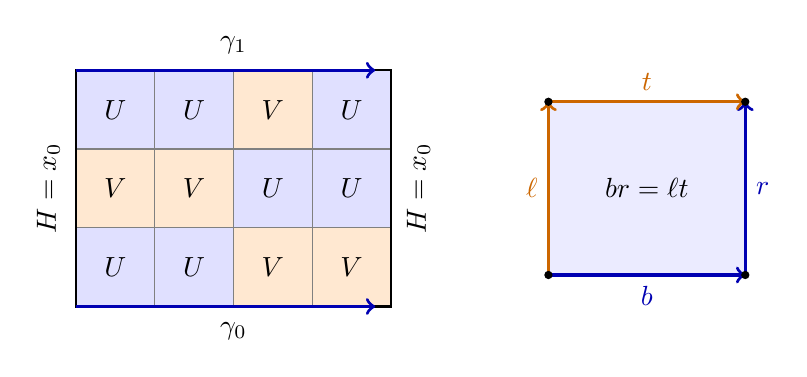
\begin{tikzpicture}[x=1cm,y=1cm]
	\foreach \x/\y in {0/0,1/0,2/1,3/1,0/2,1/2,3/2}{
		\fill[blue!12] (\x,\y) rectangle +(1,1);
	}
	\foreach \x/\y in {2/0,3/0,0/1,1/1,2/2}{
		\fill[orange!18] (\x,\y) rectangle +(1,1);
	}
	\draw[step=1,gray] (0,0) grid (4,3);
	\draw[thick] (0,0) rectangle (4,3);
	\foreach \x/\y/\s in {.5/.5/U,1.5/.5/U,2.5/.5/V,3.5/.5/V,.5/1.5/V,1.5/1.5/V,2.5/1.5/U,3.5/1.5/U,.5/2.5/U,1.5/2.5/U,2.5/2.5/V,3.5/2.5/U}{
		\node at (\x,\y) {\(\s\)};
	}
	\draw[very thick,->,blue!70!black] (0,0)--(3.8,0);
	\draw[very thick,->,blue!70!black] (0,3)--(3.8,3);
	\node[below] at (2,-.08) {\(\gamma_0\)};
	\node[above] at (2,3.08) {\(\gamma_1\)};
	\node[rotate=90] at (-.35,1.5) {\(H=x_0\)};
	\node[rotate=90] at (4.35,1.5) {\(H=x_0\)};
	\fill[blue!8] (6,.4) rectangle (8.5,2.6);
	\draw[very thick,blue!70!black,->] (6,.4)--(8.5,.4) node[midway,below] {\(b\)};
	\draw[very thick,blue!70!black,->] (8.5,.4)--(8.5,2.6) node[midway,right] {\(r\)};
	\draw[very thick,orange!80!black,->] (6,.4)--(6,2.6) node[midway,left] {\(\ell\)};
	\draw[very thick,orange!80!black,->] (6,2.6)--(8.5,2.6) node[midway,above] {\(t\)};
	\node at (7.25,1.5) {\(br=\ell t\)};
	\foreach \x/\y in {6/.4,8.5/.4,6/2.6,8.5/2.6}{
		\fill (\x,\y) circle (1.5pt);
	}
\end{tikzpicture}

	\caption[同伦方格中的道路替换]{同伦方形被细分，使每个小格的像落在一个开集中。右图把一个小格的下边后右边换为左边后上边；所有边通过连接道路接到同一基点，因而得到群等式 \(br=\ell t\)。}
	\label{g1:fig:van-kampen-grid}
\end{figure}

这个证明也给出泛性质。若 \(f_U:\pi_1(U,x_0)\to K\) 与 \(f_V:\pi_1(V,x_0)\to K\) 满足 \(f_Ui_U=f_Vi_V\)，自由积上的延拓会消去所有关系词，故唯一下降为 \(\pi_1(X,x_0)\to K\)。因此计算的关键是两边的群、交集的群和两条包含同态，而不只是三个群的抽象同构类型。

\subsection{多重交集、基点选择与推广范围}
\label{g1:subsec:0502:03}

有限图常需要同时使用好几个开集。下面给出一个条件稍强、却足以直接使用同一网格证明的多开集版本。它允许任意多个开集，但所有开集共用一个基点。

\begin{corollary}[共同基点的多开集版本]\label{g1:cor:many-set-van-kampen}
	设 \(X=\bigcup_{\alpha\in A}U_\alpha\)，每个 \(U_\alpha\) 都开且包含同一点 \(x_0\)，并且任意非空有限个 \(U_\alpha\) 的交集都道路连通。则包含映射诱导同构
	\[
		\pi_1(X,x_0)\cong
		\left(\mathop{*}_{\alpha\in A}\pi_1(U_\alpha,x_0)\right)\big/N,
	\]
	其中 \(N\) 是所有成对交集闭路在两个因子中所给元素之差
	\(i_{\alpha\beta}(\omega)i_{\beta\alpha}(\omega)^{-1}\) 的正规闭包。
\end{corollary}
\begin{proof}
	对一条道路或一个同伦方形，拉回的开覆盖仍有 Lebesgue 数，故只需要有限段或有限个小矩形。段的交点处，在两个标记的交集中选择连接道路；网格顶点处，在所有相邻小矩形标记的交集中选择连接道路，最多涉及四个开集。改变某段标记时，若它的端点还邻接其他标记，就把端点连接道路选在所有这些标记的交集中，所需交集仍是有限交。假设保证上述选择都能完成。

	其余论证逐项与双开集情形相同：连接道路改变所造成的因子在成对交集关系下相消；共同细分比较不同分段；每条公共网格边在其两侧因子中表示同一元素；逐格等式 \(br=\ell t\) 证明同伦不变。由此构造与自然同态互逆的同态，得到同构。开覆盖可以无限，并不要求 \(X\) 紧；用到紧性的只是道路和同伦的参数空间。
\end{proof}

这里要求所有有限交道路连通，是为了能直接在普通四边网格的顶点选择连接道路。更精细的版本只要求成对与三重交道路连通，并把网格错开，使每个顶点至多接触三个标记；本节的应用使用上述已证明的充分条件。一般没有公共基点、或者交集不道路连通时，需要保留多个基点之间的道路信息，不能直接套用同一个商群公式。

最小的警示就是圆周。取 \(U=S^1\setminus\{-1\}\)、\(V=S^1\setminus\{1\}\)，它们都是可缩开弧，交集却有两个道路分支。若忽略交集的道路连通条件，两个平凡群的自由积会错误地给出平凡群；而\cref{g1:thm:circle-fundamental}已经证明圆周的基本群是 \(\mathbb Z\)。从一条开弧走进另一条开弧后再返回，需要知道经过交集的哪一个分支。只有一个基点的交集基本群没有记录这个信息。

改变基点也不是把记号无条件删去。由\cref{g1:prop:basepoint-change}，道路 \(c:x_0\to x_1\) 给出
\[
	\pi_1(X,x_0)\longrightarrow\pi_1(X,x_1),\qquad
	[\gamma]\longmapsto[\bar c*\gamma*c].
\]
若分别给各个开集选了基点，计算包含同态前必须先指定把它们接到公共基点的道路。更改连接道路通常会把相应元素作共轭；这不改变“加入某条闭路的全部共轭作为关系”的正规闭包，却可能改变具体生成元写出的词。因而群的同构类型可以不依赖某些选择，展示的字母与几何闭路之间的对应仍须写清。

还须注意开性。证明中先把参数区间或方形的开覆盖细分；若把空间任意拆成两个闭子集，拉回覆盖不再提供这种细分保证。下面的图和圆盘附着计算都会明确取开邻域，再通过形变收缩把这些邻域化为易算的对象。

\subsection{图、曲面和去点空间的群展示}
\label{g1:subsec:0502:04}

先看只有边而没有面的空间。这里的有限图是把有限多个闭区间的端点附着到有限个顶点所得的商空间，允许一条边两端相同，也允许两顶点之间有多条边；连通指顶点之间可由有限边路连接。有限图带上述商拓扑，等价地可在每条边赋长度 \(1\) 后用最短边路长度定义度量：边内部的小球是区间，顶点的小球是有限条短边段接成的星形，这些正好给出商拓扑的局部开集。图因而是紧 Hausdorff 空间。

一个不含回路的连通子图称为树。若有限连通图中还有回路，删去该回路的一条边的内部不会破坏顶点间的连通；有限次删除以后得到包含所有顶点的树 \(T\)，称为\term[shengchengshu]{生成树}[spanning tree]。树中任意两顶点间恰有一条不重复顶点的边路：存在性来自连通，若有两条不同的简单边路，分岔后第一次重逢就产生回路。有限树若不止一个顶点，任一最长简单边路的两个端点都只有一条邻边，否则可延长或产生回路。逐次删除这种末端边便知，含 \(v\) 个顶点的树有 \(v-1\) 条边。

树还能形变收缩到任一指定顶点。每次选择一个不同于该顶点的末端顶点，将其唯一邻边按区间坐标线性缩到另一端，其他边保持不动；这些映射在共同端点处相容，故由有限闭集粘合连续。有限次组合便给出保持指定顶点不动的收缩。这是下面去掉树状部分时所需的实际同伦。

\begin{proposition}[有限连通图的基本群]\label{g1:prop:graph-fundamental}
	设 \(G\) 是有 \(v\) 个顶点、\(e\) 条边的有限连通图，\(T\) 是一棵生成树，\(x_0\) 是顶点。则
	\[
		\pi_1(G,x_0)\cong F_{e-v+1}.
	\]
	给每条不在 \(T\) 中的边选定方向，从 \(x_0\) 沿树走到该边起点，走过该边，再沿树返回 \(x_0\)，所得闭路给出一组自由生成元。
\end{proposition}
\begin{proof}
	若没有非树边，\(G=T\) 可缩，结论为平凡群 \(F_0\)。否则对每条非树边 \(d\)，令 \(U_d\) 包含整棵树、整条边 \(d\)，以及其他非树边两端参数长度小于 \(1/3\) 的短边段。每个顶点附近的所有短边段都被包括，所以 \(U_d\) 在图中开；这些集合覆盖 \(G\)，并都包含 \(x_0\)。

	把额外短边段各自线性缩到端点，\(U_d\) 形变收缩到 \(T\cup d\)。树中连接 \(d\) 两端的唯一路径与 \(d\) 组成一个圆周；其余边是附着在这个圆周上的有限树枝，依次收缩末端边就把 \(T\cup d\) 收缩到该圆周。若 \(x_0\) 不在圆周上，收缩时它沿树路移到圆周，再用基点变化公式，得到的生成元正是命题中说明的闭路。因此由\cref{g1:thm:circle-fundamental}及形变收缩不改变基本群，\(\pi_1(U_d,x_0)\cong\mathbb Z\)。

	两个或更多不同 \(U_d\) 的交集只含 \(T\) 及各非树边的端点短边段。缩去这些短边段，再收缩树，交集便可缩，且上述收缩保持 \(x_0\) 不动。因此所有有限交道路连通，成对交集基本群平凡。由\cref{g1:cor:many-set-van-kampen}，\(\pi_1(G,x_0)\) 是每条非树边所贡献的 \(\mathbb Z\) 的自由积。非树边数为 \(e-(v-1)\)，结论成立。
\end{proof}

例如两顶点之间的三条边组成的图有基本群 \(F_2\)。选中间一条边为树，另外两条边各给出一个生成元。虽然在纸面图上它围出两个有界区域，这些区域并不属于图本身，所以没有提供把闭路填满的同伦。往图中加入一张面，才会真正增加关系。

\begin{figure}[htbp]
	\centering
	% !TeX root = ../Book1.tex
\begin{tikzpicture}[x=1cm,y=1cm]
	\draw[very thick,blue!70!black] (0,1.5)--(3,1.5) node[midway,below] {\(T\)};
	\draw[thick,->] (0,1.5) to[bend left=55] node[midway,above] {\(d_1\)} (3,1.5);
	\draw[thick,->] (0,1.5) to[bend right=55] node[midway,below] {\(d_2\)} (3,1.5);
	\fill (0,1.5) circle (2pt) node[left] {\(x_0\)};
	\fill (3,1.5) circle (2pt);
	\node[align=center] at (1.5,-.25) {\(e=3,\ v=2\)\\\(\pi_1=F_2\)};
	\fill[blue!8] (5.5,.3) rectangle (7.9,2.7);
	\draw[thick] (5.5,.3) rectangle (7.9,2.7);
	\draw[very thick,blue!70!black,->] (5.9,.3)--(7.5,.3) node[midway,below] {\(a\)};
	\draw[very thick,blue!70!black,->] (5.9,2.7)--(7.5,2.7) node[midway,above] {\(a\)};
	\draw[very thick,orange!80!black,->] (5.5,.7)--(5.5,2.3) node[midway,left] {\(b\)};
	\draw[very thick,orange!80!black,->] (7.9,.7)--(7.9,2.3) node[midway,right] {\(b\)};
	\node[align=center] at (6.7,1.5) {附着圆盘\\\(aba^{-1}b^{-1}=1\)};
	\node at (6.7,-.3) {\(\pi_1(T^2)=\mathbb Z^2\)};
\end{tikzpicture}

	\caption[图的生成元与附着面的关系]{左图中间的蓝边是一棵生成树，其余两边分别贡献自由生成元；纸面上围出的区域不属于图。右图的方形内部则是实际加入的圆盘，按箭头识别对边后，其边界词给出关系 \(aba^{-1}b^{-1}=1\)。}
	\label{g1:fig:graph-and-cell}
\end{figure}

\begin{proposition}[附着一个圆盘]\label{g1:prop:attach-disk}
	设 \(X\) 是道路连通的紧 Hausdorff 空间，\(f:S^1\to X\) 连续，\(x_0=f(1)\)。令
	\[
		Y=X\cup_fD^2=(X\sqcup D^2)/(z\sim f(z)\text{ 对所有 }z\in S^1),
	\]
	即只把圆盘边界按 \(f\) 附着到 \(X\)。记边界闭路为 \(\beta(t)=f(e^{2\pi it})\)。则包含映射给出满同态，且
	\[
		\pi_1(Y,x_0)\cong\pi_1(X,x_0)/\langle\!\langle[\beta]\rangle\!\rangle.
	\]
\end{proposition}
\begin{proof}
	先交代这个商空间及所用收缩的连续性。圆盘内部没有识别，其像是开子空间。对 \(X\) 中的开集 \(O\)，集合
	\[
		O\ \cup\ \{ru:1-\varepsilon<r\le1,\ u\in S^1,\ f(u)\in O\}
	\]
	在商空间中给出 \(O\) 的开邻域；这里边界点已按 \(f\) 识别。若 \(X\) 中两点不同，取不交开邻域 \(O_1,O_2\)，上述邻域也不交。若一个点在圆盘内部，则取半径较大的薄边界环带把它与 \(X\) 分开；两个圆盘内部点用普通小圆盘分开。因此 \(Y\) 为 Hausdorff 空间，且由紧空间 \(X\sqcup D^2\) 的连续像而紧。相同邻域描述也表明 \(X\) 到其像为同胚。

	记圆盘中心的像为 \(o\)，取开集 \(U=Y\setminus\{o\}\) 与 \(V=\{z\in D^2:|z|<2/3\}\) 的像。它们覆盖 \(Y\)，\(V\) 为开圆盘，而交集是 \(0<|z|<2/3\) 的环带。\(U\) 形变收缩到 \(X\)：保持 \(X\) 不动，把每个 \(ru\)（\(r>0\)）送到 \(((1-t)r+t)u\)，终点 \(u\) 按附着关系就是 \(f(u)\)。在边界上公式始终给出 \(f(u)\)，所以与 \(X\) 上的恒等映射相容。为核验同伦一起连续，可注意商映射 \(q:X\sqcup D^2\to Y\) 与 \(\operatorname{id}_{[0,1]}\) 的积是紧空间到 Hausdorff 空间的连续满射，故为闭商映射；限制到开集 \(U\times[0,1]\) 的原像后仍为商映射，上述相容的连续公式遂下降为连续同伦。

	在交集中取基点 \(y_0=1/2\)，其基本群由逆时针圆周 \(t\mapsto\tfrac12e^{2\pi it}\) 生成。径向收缩把这个闭路送到 \(\beta\)；把 \(x_0\) 与 \(y_0\) 沿半径连接并使用基点变化，就得到交集群到 \(\pi_1(U)\) 的像由 \([\beta]\) 生成。另一边 \(V\) 可缩，包含同态把这个生成元送到单位元。由\cref{g1:thm:van-kampen}，商去的正是 \([\beta]\) 的正规闭包。最后沿同一半径把基点换回 \(x_0\)，便得到陈述中的包含同态及其核。
\end{proof}

为何要取正规闭包，而不只删掉整数次的 \(\beta\)？从 \(x_0\) 先沿另一条闭路 \(\eta\) 绕一段，再走圆盘边界，最后沿 \(\bar\eta\) 返回，也能利用同一张圆盘收缩。因此 \([\eta][\beta][\eta]^{-1}\) 必须同时成为单位元。有限次附着圆盘时可逐次应用上面的命题；每一步仍是紧 Hausdorff 空间，最终加入所有附着边界词的关系。

\begin{example}[三个曲面模型的群]\label{g1:exm:surface-presentations}
	环面 \(T^2\) 的基本群为 \(\mathbb Z^2\)，实射影平面 \(\mathbb RP^2\) 的基本群为 \(\mathbb Z/2\mathbb Z\)，从环面去掉一点所得空间的基本群为 \(F_2\)。
\end{example}
\begin{proof}
	在\cref{g1:thm:torus-square}的方形模型中，边界识别后成为有一个顶点、两条环边 \(a,b\) 的图。从左下角出发，逆时针沿方形边界走，依次读出
	\[
		aba^{-1}b^{-1}.
	\]
	方形的内部是一张附着到这个图上的圆盘，故附着命题与图的计算给出
	\[
		\pi_1(T^2)\cong\langle a,b\mid aba^{-1}b^{-1}=1\rangle\cong\mathbb Z^2.
	\]
	这也与\cref{g1:prop:product-fundamental}和 \(T^2=S^1\times S^1\) 的计算相合。边界词记录了具体的附着方向，不是仅凭图形有两个“洞”猜出两个交换的生成元。

	实射影平面可由闭圆盘边界上的对径点识别得到。确切地，将 \(D^2\) 同胚地送到 \(S^2\) 的上半球，再送到对径商 \(S^2/\{\pm1\}\)：每个对径类都有上半球代表，上半球内部的代表唯一，赤道上的两个对径代表恰好被识别。于是得到从圆盘边界对径商到 \(\mathbb RP^2\) 的连续双射；源空间紧，目标由\cref{g1:thm:real-projective-quotient}为 Hausdorff，故是同胚。

	边界自身的商仍是圆周，其坐标可写为 \(e^{i\theta}\mapsto e^{2i\theta}\)。所以绕圆盘边界一周在商圆周上走两周，附着词为 \(a^2\)。得到
	\[
		\pi_1(\mathbb RP^2)\cong\langle a\mid a^2=1\rangle\cong\mathbb Z/2\mathbb Z.
	\]
	最后从环面方形模型的内部去掉中心点，剩下的方形沿从中心发出的射线形变收缩到边界，边界点保持不动，所以同伦与对边识别相容。也可把方形看作圆盘后直接用附着命题证明中的 \(U\) 的径向收缩。所得图是两个圆周在一点相接，故去点环面的基本群为 \(F_2\)。去掉任意其他一点得到相同结论，因为积模型中的旋转 \((z,w)\mapsto(cz,dw)\) 可将任一点移到指定点。
\end{proof}

这些计算针对已经明确构造的曲面，没有使用曲面分类定理。更一般地，若一个多边形模型的边界识别后是一顶点图，先给图中的环边选方向，再沿多边形边界读出词 \(w\)，上述命题便给出 \(\langle a_1,\ldots,a_r\mid w=1\rangle\)。若要断言某个任意给定的曲面必属于某类多边形模型，还需要下一章的分类论证；群展示本身不承担这一任务。

\begin{proposition}[高维球面的单连通性]\label{g1:prop:sphere-simply-connected}
	对每个整数 \(k\ge2\)，球面 \(S^k\) 单连通。
\end{proposition}
\begin{proof}
	当 \(k\ge2\) 时，\(S^k\) 去掉北极或南极得到两个开集，各由球极投影同胚于 \(\mathbb R^k\)：写点为 \((x,t)\in\mathbb R^k\times\mathbb R\)，从北极投影为 \(x/(1-t)\)，逆映射为
	\[
		u\longmapsto\left(\frac{2u}{1+\lVert u\rVert^2},
		\frac{\lVert u\rVert^2-1}{1+\lVert u\rVert^2}\right).
	\]
	南极情形将末坐标变号。这两个开集可缩，交集由
	\[
		(v,t)\longmapsto(\sqrt{1-t^2}\,v,t)
	\]
	同胚于 \(S^{k-1}\times(-1,1)\)，因而道路连通。这里 \(S^{k-1}\) 道路连通可直接看出：两个不对径的单位向量用线段归一化连接，对径时先经一个不与它们共线的单位向量。两个开集道路连通且交集非空，故球面道路连通；再由 van Kampen 定理，两个平凡群的自由积再取商仍平凡，所以 \(\pi_1(S^k)=1\)。
\end{proof}

\begin{proposition}[欧氏空间去掉有限个点]\label{g1:prop:punctured-euclidean}
	设 \(P\subseteq\mathbb R^n\) 是含 \(m\) 个点的有限集合。若 \(n=2\)，则 \(\mathbb R^2\setminus P\) 道路连通，基本群同构于 \(F_m\)，可选从基点出发绕各缺失点一周再返回的闭路作为自由生成元。若 \(n\ge3\)，则 \(\mathbb R^n\setminus P\) 单连通。
\end{proposition}
\begin{proof}
	先说明单点情形。平移把缺失点移到原点，公式
	\[
		H(x,t)=\left(1-t+\frac{t}{\lVert x\rVert}\right)x
	\]
	把 \(\mathbb R^n\setminus\{0\}\) 形变收缩到 \(S^{n-1}\)。当 \(n=2\) 时得到 \(\mathbb Z\)；当 \(n\ge3\) 时，\(n-1\ge2\)，由\cref{g1:prop:sphere-simply-connected}得到单连通性。

	对一般 \(m\) 归纳，\(m=0\) 是可缩的欧氏空间。为使 \(P\) 中各点的第一坐标互不相同，考虑 \(v(t)=(1,t,\ldots,t^{n-1})\)：对任意两不同点之差 \(d\)，内积 \(\langle d,v(t)\rangle\) 是非零多项式，只有有限个实根。取 \(t\) 避开有限个点差所对应的全部实根，再以 \(v(t)\) 的方向为第一坐标轴，就得到所需坐标。取相邻的两个第一坐标之间的数 \(a<b\)，令开条带 \(a<x_1<b\) 不含缺失点，并使 \(x_1<b\) 的开半空间只含最左边的一个缺失点。于是
	\[
		U=(\{x_1<b\}\setminus P),\qquad
		V=(\{x_1>a\}\setminus P)
	\]
	覆盖补空间，交集是凸开条带。每个开半空间同胚于 \(\mathbb R^n\)，例如第一坐标可用 \(\log(b-x_1)\) 或 \(\log(x_1-a)\) 替换，其余坐标不变。因此 \(U\) 是一个点的补空间，\(V\) 对应 \(m-1\) 个点的补空间；它们由归纳假设道路连通，交集可缩。van Kampen 定理给出两基本群的自由积。平面情形为 \(\mathbb Z*F_{m-1}=F_m\)，高维情形为平凡群。

	取交集中的公共基点，并逐次沿条带及半空间中的道路连接到各个小圆周，便得到陈述中的自由生成元；道路的改变会改变所选基及其共轭表达，不改变自由群的同构类型。这个归纳同时证明了补空间道路连通，因为两个道路连通开集有非空交集。
\end{proof}

去点空间说明维数会改变绕行障碍：在平面中，一个缺失点留下一个自由生成元；在至少三维时，闭路可以借额外方向绕过该点并收缩。它也提醒我们不要把“各点绕数都为零”当成平面多点补空间中闭路可收缩的判据，自由群还保留走法的次序。相关的一般方法可参阅\cite[Section 1.2]{Hatcher2002}。
% 纲要条目排为编号小节标题，并进入目录与书签；说明段仍保留于纲要注释中。

% !TeX root = ../../Book1.tex
% 纲要标题：### 5.3 覆盖映射的提升理论
% 纲要位置：几何学计划纲要.md，第 291 行。
% 正文状态：初稿完成，未正式审核。

% 纲要内容开始
% 
% * 覆盖的局部乘积结构
% * 道路提升及唯一性
% * 同伦提升与提升判据
% * 甲板变换及其对纤维的作用
% 
% 纲要内容结束

\section{覆盖映射的提升理论}
\label{g1:sec:0503}

沿圆周连续选择一个实数角度时，可以从任意初始角度出发，并一直跟随道路；但绕圆一周以后，角度增加了 \(2\pi\)，没有回到原值。覆盖映射把这个现象推广到一般空间：底空间上的一个小邻域在上方分成若干互不相交的副本，局部选择一个副本以后，连续移动就决定了下一步该去哪里。真正需要证明的是这种局部选择能否沿整条道路延续、能否随参数连续变化，以及沿不同道路得到的选择何时一致。

\subsection{覆盖的局部乘积结构}
\label{g1:subsec:0503:01}

设想把若干张相同地图叠在一起，每张都投影到同一个区域。这里地图只是局部模型；走到区域外以后，各张地图可以重新连接，所以全空间未必是不交的若干份底空间。

\begin{definition}[覆盖映射]\label{g1:def:covering-map}
	设 \(E,X\) 为拓扑空间。连续满射 \(p:E\to X\) 称为\term[fugaiyingshe]{覆盖映射}[covering map]，如果每个 \(x\in X\) 都有开邻域 \(U\)，使
	\[
		p^{-1}(U)=\bigsqcup_{\lambda\in\Lambda}V_\lambda,
		\qquad p|_{V_\lambda}:V_\lambda\longrightarrow U
	\]
	为同胚，且各 \(V_\lambda\) 都在 \(E\) 中开。这样的 \(U\) 称为\term[junyunfugailinyu]{均匀覆盖邻域}[evenly covered neighborhood]，各 \(V_\lambda\) 称为该邻域上方的\term[fugaipian]{覆盖片}[sheet]。空间 \(X\) 称为底空间，\(E\) 称为覆盖空间；集合 \(p^{-1}(x)\) 称为点 \(x\) 上的纤维，与\secref{g1:sec:0206}中“一个指定点的逆像”的用法相同。
\end{definition}

给指标集 \(\Lambda\) 离散拓扑，映射 \(V_\lambda\ni e\mapsto(p(e),\lambda)\) 将 \(p^{-1}(U)\) 同胚地识别为 \(U\times\Lambda\)，并把 \(p\) 化为第一投影。这就是覆盖的局部乘积结构。反过来，这种与投影相容的局部乘积表示也给出定义中的分解。覆盖片是相对于所选 \(U\) 而言的，不能未经证明就把某一片延伸为整个 \(E\) 的一个分支。若连续映射在每个源点附近都限制为到目标某个开集的同胚，称它为\term[jubutongpei]{局部同胚}[local homeomorphism]；这里邻域选在源空间中，定义本身不要求满射。

\begin{proposition}[覆盖的局部性质]\label{g1:prop:covering-local-properties}
	覆盖映射 \(p:E\to X\) 是局部同胚、开映射和商映射，每个纤维带子空间拓扑时都是离散空间。若 \(X\) 局部道路连通，则 \(E\) 也局部道路连通。
\end{proposition}
\begin{proof}
	每个 \(e\in E\) 都落在某张覆盖片上，而这张片到相应开邻域的限制是同胚，故 \(p\) 为局部同胚。若 \(O\subseteq E\) 开，将 \(O\) 与所有覆盖片相交，每一交集的像都在相应 \(U\) 中开，从而在 \(X\) 中开；这些像的并就是 \(p(O)\)，所以 \(p\) 开。连续开满射是商映射：若 \(p^{-1}(A)\) 开，则 \(A=p(p^{-1}(A))\) 开；另一方向由连续性得到。

	在 \(x\) 上方，每张覆盖片恰与 \(p^{-1}(x)\) 相交于一点，所以纤维的每个单点都相对开。最后，若 \(X\) 局部道路连通，给定 \(e\) 的开邻域 \(O\)，先在一张含 \(e\) 的覆盖片 \(V\) 中看 \(O\cap V\)，再在其像内取含 \(p(e)\) 的道路连通开邻域。该邻域经 \((p|_V)^{-1}\) 的像是包含在 \(O\) 内的道路连通开邻域，证明了 \(E\) 的局部道路连通性。
\end{proof}

若纤维有 \(n\) 个点，常称覆盖在该点为 \(n\) 叶。均匀覆盖邻域内各点的纤维与同一个 \(\Lambda\) 一一对应，所以纤维基数局部不变。特别地，底空间连通时该基数在整个底空间上相同：与一个给定纤维等势的点组成开闭子集。允许无限叶，也允许覆盖空间不连通。

\begin{example}[圆周的两个覆盖]\label{g1:exm:circle-coverings}
	映射
	\[
		q:\mathbb R\longrightarrow S^1,\qquad q(t)=e^{2\pi it}
	\]
	是覆盖。确实，取 \(a\in\mathbb R\) 和 \(0<\varepsilon<1/4\)，令 \(U=q((a-\varepsilon,a+\varepsilon))\)。这是圆周开弧，并且
	\[
		q^{-1}(U)=\bigsqcup_{k\in\mathbb Z}(a-\varepsilon+k,a+\varepsilon+k).
	\]
	每个限制都是同胚：在旋转后的开弧 \(e^{-2\pi ia}U\) 上实部为正，故角度可由连续函数 \(\arctan(\operatorname{Im}z/\operatorname{Re}z)\) 恢复，再加上 \(a+k\)。每个纤维是一份整数集。

	对整数 \(n\ge1\)，映射
	\[
		p_n:S^1\longrightarrow S^1,\qquad p_n(z)=z^n
	\]
	也是覆盖。上面开弧 \(U\) 的原像由 \(n\) 条不交开弧组成，它们分别由
	\[
		z=e^{2\pi i(t+j)/n},\qquad
		a-\varepsilon<t<a+\varepsilon,\quad j=0,\ldots,n-1
	\]
	参数化；\(p_n\) 将每条开弧同胚地映到 \(U\)。所以它是 \(n\) 叶覆盖。
\end{example}

局部同胚满射还不足以保证覆盖。例如 \((0,2)\to S^1\)、\(t\mapsto e^{2\pi it}\) 处处局部同胚且满射，但 \(1\) 上只有一个原像 \(1\)，而其附近的非 \(1\) 点有两个原像，不可能有均匀覆盖邻域。另一方面，\(\mathbb C\to\mathbb C\)、\(z\mapsto z^n\) 在 \(n\ge2\) 时也不是覆盖：原点的每个邻域中都有两个不同的非零点具有相同 \(n\) 次方，故原点附近连局部单射都不成立。覆盖要求的正是这种分支现象不出现。

\subsection{道路提升及唯一性}
\label{g1:subsec:0503:02}

给定连续映射 \(f:Y\to X\)，寻找连续映射 \(\widetilde f:Y\to E\) 满足 \(p\circ\widetilde f=f\)，称为将 \(f\)\term[tisheng]{提升}[lift]到覆盖空间。它所要求的交换关系是
\[
	\begin{tikzcd}[column sep=large,row sep=large]
		& E\arrow[d,"p"]\\
		Y\arrow[ur,dashed,"\widetilde f"]\arrow[r,"f"']&X.
	\end{tikzcd}
\]
提升如果存在，通常还需指定一个点的取值。先证明这个取值会带来多强的唯一性。

\begin{lemma}[连通空间上的提升唯一性]\label{g1:lem:lift-uniqueness}
	设 \(p:E\to X\) 为覆盖，\(Y\) 连通，且连续映射 \(f_1,f_2:Y\to E\) 满足 \(p\circ f_1=p\circ f_2\)。若它们在某一点相等，则处处相等。
\end{lemma}
\begin{proof}
	令 \(A=\{y:f_1(y)=f_2(y)\}\)。对任一点 \(y\)，选 \(p(f_1(y))\) 的均匀覆盖邻域 \(U\)，并令 \(V_1,V_2\) 为分别包含 \(f_1(y),f_2(y)\) 的覆盖片。在开邻域 \(f_1^{-1}(V_1)\cap f_2^{-1}(V_2)\) 内，若 \(V_1=V_2\)，两映射由该片上 \(p\) 的单射性必相等；若 \(V_1\ne V_2\)，它们则因覆盖片不交而处处不等。因此 \(A\) 及其补集都开。由于 \(Y\) 连通且 \(A\ne\varnothing\)，有 \(A=Y\)。
\end{proof}

这里没有假设 \(E\) 为 Hausdorff 空间。相等集的闭性来自覆盖片的分离结构，而不是一般的“连续映射相等集为闭集”结论；后者通常需要目标的 Hausdorff 条件。

\begin{theorem}[道路提升]\label{g1:thm:path-lifting}
	设 \(p:E\to X\) 为覆盖，\(\alpha:[0,1]\to X\) 为道路，且 \(e_0\in E\) 满足 \(p(e_0)=\alpha(0)\)。则存在唯一道路 \(\widetilde\alpha:[0,1]\to E\)，满足
	\[
		p\circ\widetilde\alpha=\alpha,\qquad \widetilde\alpha(0)=e_0.
	\]
\end{theorem}
\begin{proof}
	唯一性由\cref{g1:lem:lift-uniqueness}及区间的连通性得到。构造时，要把道路分成有限段，使每段都落在一个均匀覆盖邻域内，然后由已确定的接点选择下一张片。

	把 \(X\) 的均匀覆盖邻域拉回到 \([0,1]\)，得到该紧度量空间的开覆盖。\cref{g1:lem:lebesgue-number}给出 \(\delta>0\)，使直径小于 \(\delta\) 的子集包含在一个覆盖成员内。取分割 \(0=t_0<t_1<\cdots<t_m=1\)，每段长度小于 \(\delta\)。于是可选均匀覆盖邻域 \(U_j\)，使 \(\alpha([t_{j-1},t_j])\subseteq U_j\)。

	在第一段，取包含 \(e_0\) 的覆盖片 \(V_1\)，定义 \(\widetilde\alpha=(p|_{V_1})^{-1}\circ\alpha\)。若前 \(j-1\) 段已定义，就取 \(U_j\) 上方包含已知端点 \(\widetilde\alpha(t_{j-1})\) 的那一片 \(V_j\)，并在第 \(j\) 段定义 \(\widetilde\alpha=(p|_{V_j})^{-1}\circ\alpha\)。两个相邻公式在接点上相同，故由有限闭集粘合\cref{g1:prop:gluing-lemma}得到连续道路。每段都满足投影等式，第一段又给出指定初值，所以所构造的道路即为所求。
\end{proof}

连续性禁止道路在同一均匀覆盖邻域的不同片之间突然跳跃；有限分割则保证每一次局部选择都能传递到下一段。对反向道路与拼接道路，唯一性立即给出相容性：提升 \(\bar\alpha\) 时若从 \(\widetilde\alpha(1)\) 出发，就得到反向道路 \(\overline{\widetilde\alpha}\)；提升 \(\alpha*\beta\) 时，先提升 \(\alpha\)，再从其终点提升 \(\beta\)，所得拼接就是整条提升。

\begin{figure}[htbp]
	\centering
	% 圆周上一周环路与实直线上的提升；上下两层属于不同空间。
\begin{tikzpicture}[x=1.3cm,y=1.15cm,>=Stealth]
	\draw[->,gray] (-0.7,2)--(3.7,2) node[right] {\(\mathbb R\)};
	\draw[very thick,GeometryBlue,->] (0,2)--(2,2);
	\fill (0,2) circle (1.7pt) node[above=4pt] {\(0\)};
	\fill (2,2) circle (1.7pt) node[above=4pt] {\(1\)};
	\node[above] at (1,2.25) {\(\widetilde\alpha(t)=t\)};
	\draw[gray] (1,0) circle (0.72);
	\draw[very thick,GeometryBlue,->] (1.72,0) arc[start angle=0,end angle=345,radius=0.72];
	\fill (1.72,0) circle (1.7pt) node[right=3pt] {\(1\in S^1\)};
	\draw[dashed,gray,->] (0,1.85)--(1.62,0.12);
	\draw[dashed,gray,->] (2,1.85)--(1.76,0.15);
	\node[right] at (2.0,1.05) {\(q\)};
	\node[below] at (1,-0.9) {\(\alpha(t)=e^{2\pi it}\)};
\end{tikzpicture}
% !TeX root = ../Book1.tex

	\caption[圆周环路的非闭提升]{在覆盖 \(q(t)=e^{2\pi it}\) 下，圆周上从 \(1\) 正向绕行一周的环路，从上方 \(0\) 出发提升为线段 \(t\mapsto t\)，终点为 \(1\)。上下同写数字 \(1\) 的点属于不同空间；上方的 \(0,1\) 则属于同一纤维。虚线仅表示这两个端点的投影。}
	\label{g1:fig:path-lift}
\end{figure}

环路的提升不一定闭合，这不是提升定理的缺陷，反而是覆盖保存的整体信息。例如对 \(q\)，从 \(a\) 出发提升 \(t\mapsto e^{2\pi i(a+kt)}\)，得到 \(t\mapsto a+kt\)；整数 \(k\) 直接记录提升终点相对于起点的位移。下面将证明，终点只依赖底空间道路的定端点同伦类。

\subsection{同伦提升与提升判据}
\label{g1:subsec:0503:03}

逐条提升一族道路还不够：若参数稍变而提升突然换片，就不能得到连续同伦。关键在于，一条固定道路只需要有限个局部公式；把参数限制在足够小的邻域内，这些公式可以一起使用。下述版本允许参数空间完全一般，不要求它连通、局部道路连通或紧。

\begin{theorem}[覆盖的同伦提升]\label{g1:thm:homotopy-lifting}
	设 \(p:E\to X\) 为覆盖，\(Y\) 为任意拓扑空间，\(H:Y\times[0,1]\to X\) 连续。若连续映射 \(h_0:Y\to E\) 满足 \(p(h_0(y))=H(y,0)\)，则存在唯一连续映射 \(\widetilde H:Y\times[0,1]\to E\)，满足
	\[
		p\circ\widetilde H=H,\qquad \widetilde H(y,0)=h_0(y).
	\]
\end{theorem}
\begin{proof}
	对每个 \(y\)，由道路提升定理，提升 \(t\mapsto H(y,t)\)，并指定起点 \(h_0(y)\)。逐点定义的这些提升给出唯一可能的函数 \(\widetilde H\)。问题只剩联合连续性，而不只是每条竖直道路的连续性。

	固定 \(y_0\in Y\)。如道路提升证明那样，选有限分割 \(0=t_0<\cdots<t_m=1\)，使每段 \(H(\{y_0\}\times[t_{j-1},t_j])\) 落在均匀覆盖邻域 \(U_j\) 中。对每个 \(j\)，存在 \(y_0\) 的开邻域 \(N_j\)，满足
	\[
		H(N_j\times[t_{j-1},t_j])\subseteq U_j.
	\]
	为说明这一点，对每个 \(t\in[t_{j-1},t_j]\)，用 \(H^{-1}(U_j)\) 的开放性选一个含 \((y_0,t)\) 的乘积开邻域，再由参数闭区间的紧性选有限个覆盖它；取这些邻域在 \(Y\) 方向的有限交即可。再取所有 \(N_j\) 的交，得到可同时处理全部时间段的开邻域 \(N\)。

	令 \(V_1\) 为 \(U_1\) 上方包含 \(h_0(y_0)\) 的片。由 \(h_0\) 连续，缩小 \(N\) 后有 \(h_0(N)\subseteq V_1\)，所以在 \(N\times[t_0,t_1]\) 上可用连续公式 \((p|_{V_1})^{-1}\circ H\)。这个公式在 \(t_1\) 处给出连续的端点函数。令 \(V_2\) 为 \(U_2\) 上方包含该函数在 \(y_0\) 处取值的片，再次缩小 \(N\)，使全部这些端点都在 \(V_2\) 内，然后在下一段用 \((p|_{V_2})^{-1}\circ H\)。照此继续有限次；此前的公式限制到更小的 \(N\) 上仍有效。

	最终在某个含 \(y_0\) 的开邻域 \(N\) 上，得到有限段连续公式，它们在每个接点对全部 \(y\in N\) 都一致。有限闭集粘合引理说明它们合成 \(N\times[0,1]\) 上的连续映射。对每个固定 \(y\)，该映射都是具有指定初值的道路提升，所以由唯一性，它恰等于先前逐点定义的 \(\widetilde H\)。这样的 \(N\) 覆盖 \(Y\)，故 \(\widetilde H\) 联合连续。任意另一个满足条件的提升在每条竖直道路上相等，因而全局相等。
\end{proof}

\begin{corollary}[定端点同伦的提升]\label{g1:cor:lifted-path-homotopy}
	设 \(p:E\to X\) 为覆盖，\(\alpha,\beta\) 是从 \(x_0\) 到 \(x_1\) 的定端点同伦道路。若两者的提升都从同一点 \(e_0\in p^{-1}(x_0)\) 出发，则它们终点相同，并且在 \(E\) 中定端点同伦。
\end{corollary}
\begin{proof}
	设 \(H(s,t)\) 为该同伦，其中 \(s\) 是同伦参数、\(t\) 是道路参数，故 \(H(s,0)=x_0\)、\(H(s,1)=x_1\)。用初始提升 \(s\mapsto e_0\) 提升 \(H\)。每条道路 \(\widetilde H(s,-)\) 从 \(e_0\) 出发，而终点函数 \(s\mapsto\widetilde H(s,1)\) 连续且取值于离散纤维 \(p^{-1}(x_1)\)。区间连通，连续像也连通，离散空间的连通子集至多含一点，因此该终点函数恒定。于是提升同伦的两端都固定，且由道路提升唯一性，其边界道路正是指定的两条提升。
\end{proof}

\begin{proposition}[覆盖诱导的基本群单射]\label{g1:prop:covering-pi1-injective}
	设 \(p:E\to X\) 为覆盖，\(e_0\in E\)，\(x_0=p(e_0)\)。则
	\[
		p_*:\pi_1(E,e_0)\longrightarrow\pi_1(X,x_0)
	\]
	为单射。
\end{proposition}
\begin{proof}
	由\cref{g1:prop:homotopy-functor}，\(p_*\) 是群同态，只需证明其核平凡。设 \(E\) 中基于 \(e_0\) 的环路 \(\gamma\) 满足 \(p\circ\gamma\) 定端点同伦于 \(x_0\) 处的常值道路。将这一同伦从起点 \(e_0\) 提升。由\cref{g1:cor:lifted-path-homotopy}，所得同伦固定两端；第一条边界提升是 \(\gamma\)，另一条边界提升是 \(e_0\) 处的常值道路，因为后者已是常值底道路的一个提升。因此 \([\gamma]=1\)，单射性成立。
\end{proof}

\begin{corollary}[环路提升的闭合判据]\label{g1:cor:closed-lift-criterion}
	设 \(p:(E,e_0)\to(X,x_0)\) 为带指定点的覆盖。基于 \(x_0\) 的环路 \(\alpha\) 从 \(e_0\) 出发的提升闭合，当且仅当
	\[
		[\alpha]\in p_*\pi_1(E,e_0).
	\]
\end{corollary}
\begin{proof}
	若提升 \(\widetilde\alpha\) 闭合，则它代表 \(\pi_1(E,e_0)\) 的元素，且 \(p_*[\widetilde\alpha]=[\alpha]\)。反过来，若 \([\alpha]=p_*[\gamma]\)，其中 \(\gamma\) 是 \(E\) 中基于 \(e_0\) 的环路，则 \(\alpha\) 与 \(p\circ\gamma\) 定端点同伦。从 \(e_0\) 出发的两条提升由\cref{g1:cor:lifted-path-homotopy}有相同终点，而后一提升就是环路 \(\gamma\)，所以前一提升也闭合。
\end{proof}

对于圆周的 \(n\) 叶覆盖 \(p_n\)，基本群在绕数同构 \(\pi_1(S^1,1)\cong\mathbb Z\) 下由 \(k\mapsto nk\) 给出：生成环路 \(t\mapsto e^{2\pi it}\) 与 \(p_n\) 复合后绕行 \(n\) 周。因此，一个圆周环路从 \(1\) 出发的提升闭合，恰好当它的绕数被 \(n\) 整除。这里使用的绕数同构见\cref{g1:thm:circle-fundamental}。

\ProseParagraphBreak

现在考虑整个映射 \(f:Y\to X\) 的提升。可以从 \(y_0\) 沿道路走到每个 \(y\)，提升其像，并用提升终点定义 \(\widetilde f(y)\)。可能出现的障碍是：沿两条不同道路抵达同一点时，得到的终点不同。把一条道路与另一条的反路拼起来，这一障碍便变成环路提升能否闭合的问题。

\begin{theorem}[映射的提升判据]\label{g1:thm:lifting-criterion}
	设 \(p:(E,e_0)\to(X,x_0)\) 为覆盖，\(Y\) 为道路连通且局部道路连通的空间，\(y_0\in Y\)，连续映射 \(f:Y\to X\) 满足 \(f(y_0)=x_0\)。存在连续提升 \(\widetilde f:Y\to E\) 满足 \(\widetilde f(y_0)=e_0\)，当且仅当
	\[
		f_*\pi_1(Y,y_0)\subseteq p_*\pi_1(E,e_0).
	\]
	若提升存在，则它唯一。
\end{theorem}
\begin{proof}
	必要性来自函子性：若 \(f=p\circ\widetilde f\)，则 \(f_*=p_*\circ\widetilde f_*\)，故左边的像包含于右边。唯一性来自\cref{g1:lem:lift-uniqueness}，因为道路连通蕴含连通。

	设子群包含关系成立。对每个 \(y\)，取道路 \(\alpha_y\) 从 \(y_0\) 到 \(y\)，把 \(f\circ\alpha_y\) 从 \(e_0\) 提升，并以其终点定义 \(\widetilde f(y)\)。下面分别检查选择无关性与连续性。

	若 \(\beta_y\) 是另一选择，则 \(\alpha_y*\bar\beta_y\) 为基于 \(y_0\) 的环路。假设保证其像的同伦类属于 \(p_*\pi_1(E,e_0)\)，故由\cref{g1:cor:closed-lift-criterion}，它从 \(e_0\) 出发的提升闭合。该提升先走 \(f\circ\alpha_y\) 的提升，再提升 \(f\circ\bar\beta_y\)，最终回到 \(e_0\)。反转第二段，就得到从 \(e_0\) 出发的 \(f\circ\beta_y\) 的提升，且终点正是第一段的终点。道路提升唯一性于是说明两种选择给出相同的 \(\widetilde f(y)\)。取常值道路还说明 \(\widetilde f(y_0)=e_0\)，而构造直接给出 \(p\circ\widetilde f=f\)。

	固定 \(y\)，取 \(f(y)\) 的均匀覆盖邻域 \(U\)。由 \(Y\) 局部道路连通，可在开集 \(f^{-1}(U)\) 内取含 \(y\) 的道路连通开邻域 \(V\)。令 \(W\) 为 \(U\) 上方含 \(\widetilde f(y)\) 的片。对任意 \(z\in V\)，选完全位于 \(V\) 的道路 \(\delta\) 从 \(y\) 到 \(z\)，并用 \(\alpha_y*\delta\) 作为定义 \(\widetilde f(z)\) 的道路。其后一段的像位于 \(U\)，故从 \(\widetilde f(y)\) 出发的提升为 \((p|_W)^{-1}\circ f\circ\delta\)。因此
	\[
		\widetilde f|_V=(p|_W)^{-1}\circ f|_V,
	\]
	右端连续。这对每个 \(y\) 都成立，所以 \(\widetilde f\) 连续。
\end{proof}

道路连通性用于从一个基点到达所有点，局部道路连通性则用于最后的连续性证明：它让附近各点的比较道路始终留在一个均匀覆盖邻域的原像内。两者在证明中承担不同任务。特别地，若 \(Y\) 道路连通、局部道路连通且单连通，子群条件自动成立，任何这样的 \(f\) 在指定初值以后都能唯一提升。

\subsection{甲板变换及其对纤维的作用}
\label{g1:subsec:0503:04}

在覆盖 \(q:\mathbb R\to S^1\) 中，整数平移改变了实数角度，却不改变底空间的点。一般覆盖也可能有这样的对称性：它在上方交换点，而投影后完全看不出变化。

\begin{definition}[甲板变换]\label{g1:def:deck-transformation}
	设 \(p:E\to X\) 为覆盖。满足 \(p\circ h=p\) 的同胚 \(h:E\to E\) 称为 \(p\) 的\term[jiabanbianhuan]{甲板变换}[deck transformation]，也称覆盖变换。所有甲板变换在函数通常复合
	\[
		(hk)(e)=h(k(e))
	\]
	下组成群，记为 \(\operatorname{Deck}(p)\)。
\end{definition}

确实，恒等映射满足投影等式，两个这样的同胚复合仍满足等式；从 \(p\circ h=p\) 右复合 \(h^{-1}\)，又得 \(p\circ h^{-1}=p\)，所以逆映射也在其中。每个甲板变换保持每个纤维，因而在纤维上给出置换。

\begin{proposition}[甲板变换由一点确定]\label{g1:prop:deck-determined}
	设 \(p:E\to X\) 为覆盖，且 \(E\) 非空连通。若两个甲板变换在某一点相等，则它们相同。特别地，非恒等甲板变换没有不动点；对任意 \(e_0\in E\)，映射
	\[
		\operatorname{Deck}(p)\longrightarrow p^{-1}(p(e_0)),
		\qquad h\longmapsto h(e_0)
	\]
	为单射。
\end{proposition}
\begin{proof}
	任意两个甲板变换都是映射 \(p:E\to X\) 的提升，因此可直接使用\cref{g1:lem:lift-uniqueness}。取其中一个为恒等映射，就得到不动点结论；再固定 \(e_0\)，就得到所写映射的单射性。
\end{proof}

群在集合上的作用称为自由的，是指只有单位元能固定一个点。因此在连通覆盖空间上，甲板变换群的作用自由；但自由不等于传递，不能据此断言同一纤维中的任意两点都能由某个甲板变换互换。后一性质将在下一节与正规子群联系起来。若底空间局部道路连通，则\cref{g1:prop:covering-local-properties}与\cref{g1:thm:locally-path-components}还说明：覆盖空间的连通分支就是道路分支；这里的唯一性命题本身则只需连通。

\begin{example}[圆周覆盖的甲板变换群]\label{g1:exm:circle-deck-groups}
	对于 \(q:\mathbb R\to S^1\)，整数平移 \(T_k(t)=t+k\) 都是甲板变换。反过来，若 \(h\) 是甲板变换，则 \(q(h(t))=q(t)\) 意味着 \(h(t)-t\in\mathbb Z\)。函数 \(t\mapsto h(t)-t\) 连续，\(\mathbb R\) 连通而 \(\mathbb Z\) 离散，故它恒为某个整数 \(k\)。所以全部甲板变换恰为 \(T_k\)，且
	\[
		T_k\circ T_\ell=T_{k+\ell},\qquad \operatorname{Deck}(q)\cong\mathbb Z.
	\]

	对于 \(p_n:S^1\to S^1\)，令 \(\zeta=e^{2\pi i/n}\)。旋转 \(R_j(z)=\zeta^jz\) 是甲板变换。反过来，投影等式给出 \((h(z)/z)^n=1\)，所以连续函数 \(h(z)/z\) 取值于有限离散集 \(\{1,\zeta,\ldots,\zeta^{n-1}\}\)。圆周道路连通，故该函数恒定；于是 \(h=R_j\)，且
	\[
		\operatorname{Deck}(p_n)\cong\mathbb Z/n\mathbb Z.
	\]
	这两个例子的甲板变换都在每个纤维上传递，但这一事实来自上述具体计算。
\end{example}

还有一种纤维置换来自在底空间走环路并取提升终点。它与甲板变换的来源不同，却彼此相容：若 \(\widetilde\alpha_e\) 是从 \(e\) 出发的道路提升，那么 \(h\circ\widetilde\alpha_e\) 是从 \(h(e)\) 出发的同一道路的提升，因而
\[
	h\bigl(\widetilde\alpha_e(1)\bigr)
	=\widetilde\alpha_{h(e)}(1).
\]
这一等式只用了提升唯一性。到\secref{g1:sec:0505}中，我们会将取提升终点的操作组织成基本群在纤维上的右作用，并用它重建覆盖。

% !TeX root = ../../Book1.tex
% 纲要标题：### 5.4 万有覆盖与分类定理
% 纲要位置：几何学计划纲要.md，第 298 行。
% 正文状态：初稿；尚未正式审核。

% 纲要内容开始
% 
% * 道路类构造和拓扑的定义
% * 局部假设保证覆盖性质
% * 带基点连通覆盖与子群的对应
% * 不带基点的共轭类及正规覆盖
% * 局部假设失败时分类论证在哪里中断
% 
% 纲要内容结束

\section{万有覆盖与分类定理}
\label{g1:sec:0504}

沿圆周行走时，只记录终点会丢掉已经绕过的圈数；把道路提到实线上，这段历史便保留在终点的整数偏移中。一般空间也可以尝试保留从某个固定点出发的全部道路历史。不过，连续变形不应产生新的历史，所以真正要记录的是定端点同伦类。这样得到的集合是否仍能在每一点附近看起来像原空间，正是本节首先要解决的问题。解决以后，覆盖的不同之处就可以解释为：允许把哪些环路的历史遗忘掉。

\subsection{道路类构造和拓扑的定义}
\label{g1:subsec:0504:01}

局部收缩条件有两种不同的范围。邻域中的环路能够在整个空间中缩掉，并不表示它能够在这个邻域内部缩掉。

\begin{definition}[半局部单连通]\label{g1:def:semilocally-simply-connected}
	设 \(X\) 为拓扑空间。如果每个 \(x\in X\) 都有开邻域 \(U\)，使每条以 \(x\) 为基点、完全位于 \(U\) 的环路在 \(X\) 中定基点零伦，即包含映射诱导的同态 \(\pi_1(U,x)\to\pi_1(X,x)\) 为零，就称该空间为\term[banjubudanliantong]{半局部单连通}[semilocally simply connected]。若每一点都有由单连通开邻域组成的邻域基，则称 \(X\)\term[jubudanliantong]{局部单连通}[locally simply connected]。
\end{definition}

局部单连通蕴含局部道路连通与半局部单连通；本节的分类定理只要求后两项。若 \(X\) 局部道路连通且半局部单连通，则每个开邻域 \(O\ni x\) 都包含一个道路连通开邻域 \(U\ni x\)，使 \(U\) 中的全部环路在 \(X\) 中零伦。事实上，先取半局部条件中的邻域 \(W\)，再在 \(W\cap O\) 内取道路连通开邻域 \(U\)。以 \(x\) 为基点的结论成立；以其他 \(y\in U\) 为基点的环路，可以沿 \(U\) 内一条从 \(x\) 到 \(y\) 的道路搬回 \(x\)，由\cref{g1:prop:basepoint-change}得到同样结论。下文把这样的道路连通开集 \(U\) 简称为好邻域；它不必本身单连通。

固定 \(x_0\in X\)。令 \(\widetilde X\) 为所有从 \(x_0\) 出发的道路的定端点同伦类所成的集合，定义
\[
	\widetilde x_0=[e_{x_0}],\qquad p:\widetilde X\longrightarrow X,\qquad p([\alpha])=\alpha(1).
\]
这里 \(e_{x_0}\) 是常值道路，符号 \([\alpha]\) 包含终点信息：不同终点的道路不可能代表同一个点。如何描述 \([\alpha]\) 附近的点？合理的选择是保留已有道路，只允许在它的末端追加一小段道路。若 \(U\) 是包含 \(\alpha(1)\) 的好邻域，令
\[
	B([\alpha],U)=\{[\alpha*\beta]:\beta(0)=\alpha(1),\ \beta(I)\subseteq U\}.
\]
沿用全章约定，\(\alpha*\beta\) 表示先走 \(\alpha\)，再走 \(\beta\)。改变 \(\alpha\) 的同伦代表不改变上述集合，因为道路拼接与定端点同伦相容，见\cref{g1:prop:path-classes}。

\begin{lemma}[道路类的基本邻域]\label{g1:lem:path-class-basis}
	设 \(X\) 道路连通、局部道路连通且半局部单连通，固定 \(x_0\in X\)。令 \(\widetilde X\) 为从 \(x_0\) 出发的道路的定端点同伦类集合，\(p([\alpha])=\alpha(1)\)。对含 \(\alpha(1)\) 的道路连通开集 \(U\)，要求其中所有基于 \(\alpha(1)\) 的环路在 \(X\) 中零伦，并记 \(B([\alpha],U)=\{[\alpha*\beta]:\beta:[0,1]\to U,\ \beta(0)=\alpha(1)\}\)。所有 \(B([\alpha],U)\) 构成 \(\widetilde X\) 的一个拓扑基；在此拓扑下，限制映射 \(p:B([\alpha],U)\to U\) 是同胚。
\end{lemma}
\begin{proof}
	每个 \([\alpha]\) 都属于这样的集合，因为可以追加常值道路。若 \([\delta]\in B([\alpha],U)\cap B([\gamma],V)\)，取包含 \(\delta(1)\) 的好邻域 \(W\subseteq U\cap V\)。由 \([\delta]=[\alpha*\beta]\)、\(\beta(I)\subseteq U\)，在 \(\delta\) 后追加一条位于 \(W\) 的道路，仍然得到 \(B([\alpha],U)\) 中的点；对 \(V\) 同理。所以
	\[
		B([\delta],W)\subseteq B([\alpha],U)\cap B([\gamma],V),
	\]
	这就验证了拓扑基的交集条件。

	限制映射满射，因为 \(U\) 道路连通。若 \(\beta,\beta'\) 从 \(\alpha(1)\) 出发并在 \(U\) 内到达同一个点，则 \(\beta*\bar\beta'\) 是 \(U\) 中的环路，在 \(X\) 中零伦。因此 \(\alpha*\beta\) 与 \(\alpha*\beta'\) 定端点同伦，限制映射也单射。这是好邻域条件的第一次关键使用：追加道路的终点已经决定了追加后的历史。

	对 \(X\) 中开集 \(O\) 及任意 \([\delta]\in p^{-1}(O)\)，在 \(O\) 内取 \(\delta(1)\) 的好邻域 \(W\)，则 \(B([\delta],W)\subseteq p^{-1}(O)\)。故 \(p\) 连续。另一方面，\(p\) 将每个基元素 \(B([\delta],W)\) 映为开集 \(W\)，因而是开映射。限制到一个开基元素后，仍是开映射；所以刚才得到的连续双射 \(B([\alpha],U)\to U\) 是同胚。
\end{proof}

这个拓扑记录道路的同伦历史：一个基本邻域保留已有道路，允许在末端追加位于 \(U\) 内的一小段道路。

\subsection{局部假设保证覆盖性质}
\label{g1:subsec:0504:02}

终点映射在每个基本邻域上已经是同胚。要使它成为单连通覆盖，还要证明同一底邻域上方互不相同的基本邻域彼此不交，并把总空间的环路转回道路类来计算。

\begin{definition}[万有覆盖]\label{g1:def:universal-cover}
	覆盖映射 \(p:\widetilde X\to X\) 的总空间若单连通，即非空、道路连通且基本群平凡，则称它为 \(X\) 的\term[wanyoufugai]{万有覆盖}[universal covering]。
\end{definition}

\begin{theorem}[道路类构造万有覆盖]\label{g1:thm:path-class-universal-cover}
	设 \(X\) 道路连通、局部道路连通且半局部单连通，\(x_0\in X\)。令 \(\widetilde X\) 为从 \(x_0\) 出发的道路的定端点同伦类集合。称道路连通开集 \(U\) 为好邻域，是指其中的环路在 \(X\) 中均为零伦；以 \(B([\alpha],U)=\{[\alpha*\beta]:\beta:[0,1]\to U,\ \beta(0)=\alpha(1)\}\) 为基赋予 \(\widetilde X\) 拓扑，其中 \(U\) 遍历含 \(\alpha(1)\) 的好邻域。记 \(\widetilde x_0=[e_{x_0}]\)、\(p([\alpha])=\alpha(1)\)。则 \(p:(\widetilde X,\widetilde x_0)\to(X,x_0)\) 是万有覆盖，每个好邻域都被 \(p\) 均匀覆盖。
\end{theorem}
\begin{proof}
	先固定好邻域 \(U\) 及 \(u\in U\)。在 \(p^{-1}(u)\) 中的每个道路类 \([\alpha]\) 上取基本邻域 \(B([\alpha],U)\)。这些集合覆盖 \(p^{-1}(U)\)：若 \([\eta]\) 的终点是 \(z\in U\)，取 \(U\) 内从 \(u\) 到 \(z\) 的道路 \(\beta\)，则 \([\eta*\bar\beta]\in p^{-1}(u)\)，且 \([\eta]\in B([\eta*\bar\beta],U)\)。

	不同的 \([\alpha],[\alpha']\in p^{-1}(u)\) 给出互不相交的基本邻域。否则可写 \([\alpha*\beta]=[\alpha'*\beta']\)，其中 \(\beta,\beta'\) 在 \(U\) 内由 \(u\) 到达同一点。环路 \(\beta*\bar\beta'\) 在 \(X\) 中零伦，故消去末端道路后得到 \([\alpha]=[\alpha']\)。结合\cref{g1:lem:path-class-basis}中的局部同胚，得到
	\[
		p^{-1}(U)=\coprod_{[\alpha]\in p^{-1}(u)}B([\alpha],U).
	\]
	道路连通性还保证 \(p\) 满射，所以这确实是覆盖映射。

	下面证明总空间道路连通。对任意道路 \(\alpha\) 定义初段 \(\alpha_t(s)=\alpha(ts)\)，则
	\[
		\widetilde\alpha(t)=[\alpha_t],\qquad 0\le t\le1
	\]
	从 \(\widetilde x_0\) 走到 \([\alpha]\)。它连续：在任意 \(t_0\) 附近，取好邻域 \(U\ni\alpha(t_0)\)，再把参数区间缩小，使相应的道路小段都在 \(U\) 内。无论 \(t\ge t_0\) 还是 \(t\le t_0\)，\([\alpha_t]\) 都可由 \([\alpha_{t_0}]\) 追加这段道路或其反路得到。因此在此区间内 \(\widetilde\alpha\) 等于局部逆 \((p|_{B([\alpha_{t_0}],U)})^{-1}\circ\alpha\)，从而连续。

	最后设 \(\lambda\) 是 \(\widetilde X\) 中以 \(\widetilde x_0\) 为基点的环路，令 \(\alpha=p\circ\lambda\)。上面的初段构造给出 \(\alpha\) 从 \(\widetilde x_0\) 出发的提升；由\cref{g1:thm:path-lifting}的唯一性，它就是 \(\lambda\)。因此 \([\alpha]=\widetilde\alpha(1)=\widetilde x_0\)，即 \(\alpha\) 在 \(X\) 中零伦。由\cref{g1:prop:covering-pi1-injective}，覆盖诱导的 \(p_*\) 是单射，所以 \([\lambda]=1\)。这证明了 \(\widetilde X\) 单连通。
\end{proof}

这个证明显示了两个局部条件的不同职责。局部道路连通使好邻域足够多，能够恢复 \(X\) 的原拓扑；半局部单连通则使每片基本邻域不会因绕小圈而在同一个终点上产生多个历史。

\begin{corollary}[万有覆盖向任意连通覆盖的映射]\label{g1:cor:universal-cover-map}
	设 \(X\) 为局部道路连通拓扑空间，\(x_0\in X\)，\(p:(\widetilde X,\widetilde x_0)\to(X,x_0)\) 是万有覆盖（其道路类构造见\cref{g1:thm:path-class-universal-cover}），\(q:(E,e_0)\to(X,x_0)\) 是连通覆盖。存在唯一连续映射 \(F:\widetilde X\to E\)，使 \(qF=p\)、\(F(\widetilde x_0)=e_0\)；这个 \(F\) 本身也是满射覆盖映射。
	\[
		\begin{tikzcd}
			(\widetilde X,\widetilde x_0)\arrow[rr,dashed,"F"]\arrow[dr,"p"']&&(E,e_0)\arrow[dl,"q"]\\
			&(X,x_0)&
		\end{tikzcd}
	\]
\end{corollary}
\begin{proof}
	覆盖的局部同胚性质使 \(E\) 与 \(\widetilde X\) 局部道路连通；因此连通的 \(E\) 道路连通，见\cref{g1:thm:locally-path-components}。因为 \(\pi_1(\widetilde X)=1\)，\cref{g1:thm:lifting-criterion}的子群包含条件自动满足，给出所需唯一映射。任取 \(e\in E\)，沿 \(E\) 中从 \(e_0\) 到 \(e\) 的道路投影，再提升到 \(\widetilde X\)。由提升唯一性，所得末端映到 \(e\)，所以 \(F\) 满射。

	在 \(X\) 中取一个道路连通开邻域 \(U\)，使它同时被 \(p,q\) 均匀覆盖。\(p\) 的每一片道路连通，故其在 \(F\) 下的像落在 \(q\) 的一片中，且在这两片上 \(F=(q|_{\text{该片}})^{-1}\circ p\)，是同胚。对 \(q\) 的任一片，其逆像便是若干这样的 \(p\) 的片的不交并。这说明 \(F\) 是覆盖映射。
\end{proof}

\subsection{带基点连通覆盖与子群的对应}
\label{g1:subsec:0504:03}

令 \(G=\pi_1(X,x_0)\)。前节已经说明，一个带基点覆盖 \(q:(E,e_0)\to(X,x_0)\) 决定子群 \(q_*\pi_1(E,e_0)\le G\)：它恰好收集那些从 \(e_0\) 出发后仍回到 \(e_0\) 的环路类。现在反过来，从指定子群 \(H\le G\) 出发构造覆盖。两条道路 \(\alpha,\beta\) 应被认为具有相同历史，当且仅当它们终点相同，而且相差的环路 \(\alpha*\bar\beta\) 属于 \(H\)。也就是说，\(H\) 指定了允许遗忘的环路。

\begin{theorem}[子群对应的覆盖]\label{g1:thm:subgroup-covering}
	设 \(X\) 道路连通、局部道路连通且半局部单连通，\(x_0\in X\)，\(H\le G=\pi_1(X,x_0)\)。在从 \(x_0\) 出发的道路集合上规定
	\[
		\alpha\sim_H\beta\quad\Longleftrightarrow\quad
		\alpha(1)=\beta(1)\ \text{且}\ [\alpha*\bar\beta]\in H.
	\]
	以 \([\alpha]_H\) 记等价类，令 \(E_H\) 为这些等价类的集合，\(e_H=[e_{x_0}]_H\)。以
	\[
		B_H([\alpha]_H,U)=\{[\alpha*\beta]_H:\beta:[0,1]\to U,\ \beta(0)=\alpha(1)\}
	\]
	为基赋予拓扑，其中 \(U\) 遍历含 \(\alpha(1)\) 的道路连通开邻域，且 \(U\) 中所有基于 \(\alpha(1)\) 的环路均在 \(X\) 中零伦。则终点映射 \(p_H:(E_H,e_H)\to(X,x_0)\) 是连通覆盖，且
	\[
		(p_H)_*\pi_1(E_H,e_H)=H,\qquad p_H^{-1}(x_0)\cong H\backslash G=\{Hg:g\in G\}.
	\]
	尤其覆盖的叶数为子群指数 \([G:H]\)，允许此数无限。
\end{theorem}
\begin{proof}
	关系自反、对称分别来自单位元与取逆。若 \(\alpha\sim_H\beta\)、\(\beta\sim_H\gamma\)，则
	\[
		[\alpha*\bar\gamma]=[\alpha*\bar\beta]\,[\beta*\bar\gamma]\in H,
	\]
	其中消去 \(\bar\beta*\beta\) 用的是道路类的拼接与逆关系。因此这是等价关系；特别地，同伦的道路必等价。若 \([\alpha]_H=[\alpha']_H\)，追加同一条 \(\beta\) 不改变等价性，因为 \([\alpha*\beta*\bar\beta*\bar\alpha']=[\alpha*\bar\alpha']\)。于是基元素的定义不依赖代表。

	基的交集条件与\cref{g1:lem:path-class-basis}相同：若 \([\delta]_H\) 在两个基元素中，在两好邻域交内取更小好邻域 \(W\)，则 \(B_H([\delta]_H,W)\) 同时包含在二者之内。每个 \(B_H([\alpha]_H,U)\to U\) 满射。若两个追加道路终点相同，它们在 \(U\) 中相差的环路在 \(X\) 中为单位元，因而属于 \(H\)，故此限制映射单射。它的连续性与开性也由同一基论证得到，所以是同胚。

	固定 \(u\in U\)，这些基元素在 \([\alpha]_H\) 遍历 \(p_H^{-1}(u)\) 时覆盖 \(p_H^{-1}(U)\)。若其中两片相交，则有 \([\alpha*\beta]_H=[\alpha'*\beta']_H\)，其中 \(\beta,\beta'\) 都在 \(U\) 内由 \(u\) 到达同一点。由于 \(\beta*\bar\beta'\) 在 \(X\) 中零伦，等价条件化为 \([\alpha*\bar\alpha']\in H\)，即两个索引本来就相同。因此这些片互不相交，\(p_H\) 是覆盖。初段道路 \(t\mapsto[\alpha_t]_H\) 的连续性由局部逆证明，故 \(E_H\) 道路连通。

	以 \(x_0\) 为基点的环路 \(\gamma\) 从 \(e_H\) 出发提升后终点为 \([\gamma]_H\)，它等于 \(e_H\) 当且仅当 \([\gamma]\in H\)。\cref{g1:cor:closed-lift-criterion}告诉我们，闭提升的环路类恰为 \((p_H)_*\pi_1(E_H,e_H)\)，所以该子群正是 \(H\)。纤维内的道路全是环路；若其类为 \(g,k\in G\)，等价条件为 \(gk^{-1}\in H\)，等价于 \(Hg=Hk\)。这给出所述纤维对应。其他纤维与此纤维之间可沿一条道路提升得到双射，故叶数恒为 \([G:H]\)。
\end{proof}

\begin{theorem}[带基点的连通覆盖分类]\label{g1:thm:based-covering-classification}
	设 \(X\) 道路连通、局部道路连通且半局部单连通，\(x_0\in X\)。带基点连通覆盖 \(q:(E,e_0)\to(X,x_0)\) 的等价类与 \(G=\pi_1(X,x_0)\) 的子群一一对应；这里等价指保持基点且与投影交换的同胚。对应把 \((E,e_0)\) 送到 \(q_*\pi_1(E,e_0)\)，逆对应把子群 \(H\le G\) 送到满足 \(q_*\pi_1(E,e_0)=H\) 的唯一带基点连通覆盖等价类。
\end{theorem}
\begin{proof}
	给定覆盖，令 \(H=q_*\pi_1(E,e_0)\)。总空间 \(E\) 局部道路连通，且连通，因而道路连通。定义 \(F:E_H\to E\)：把 \([\alpha]_H\) 送到 \(\alpha\) 从 \(e_0\) 出发的提升终点。需要证明，此终点恰好只忘掉 \(H\) 中的历史。

	若 \(\alpha,\beta\) 有相同终点，则其提升终点相同，当且仅当 \(\alpha*\bar\beta\) 有从 \(e_0\) 出发的闭提升。一方向可以直接把两条提升拼接；反方向把闭提升分为前后两段，反转后半段，再用 \(\beta\) 的提升唯一性。由闭提升判据，这又等价于 \([\alpha*\bar\beta]\in H\)。所以 \(F\) 良定义且单射。任意 \(e\in E\) 可沿 \(E\) 中一条从 \(e_0\) 到 \(e\) 的道路到达，取其投影就得 \(F\) 的一个原像，因此 \(F\) 满射。

	对 \([\alpha]_H\)，取包含 \(\alpha(1)\) 的好邻域 \(U\)，并使它被 \(q\) 均匀覆盖。在 \(B_H([\alpha]_H,U)\) 上，\(F\) 就是 \(p_H\) 后接经过 \(F([\alpha]_H)\) 的那片的局部逆。因此 \(F\) 局部为同胚，进而是同胚，且 \(qF=p_H\)、\(F(e_H)=e_0\)。

	如果两个带基点覆盖等价，等价同胚诱导基本群同构，故它们在 \(G\) 中的像子群相同；反过来，若像子群相同，上述构造说明它们都与同一个 \(E_H\) 等价。最后，\cref{g1:thm:subgroup-covering}保证每个子群确实出现，完成一一对应的证明。
\end{proof}

\(H=\{1\}\) 时，上述构造就是万有覆盖；\(H=G\) 时，所有同终点道路都等价，得到恒等覆盖 \(X\to X\)。子群越大，允许遗忘的历史越多，覆盖中的点就越少。万有覆盖的“万有”对应\cref{g1:cor:universal-cover-map}所述的映射性质。

\subsection{不带基点的共轭类及正规覆盖}
\label{g1:subsec:0504:04}

同一个覆盖若换了纤维中的起点，能够闭合的环路集合也可能改变。为看清改变方式，暂将从 \(e\in q^{-1}(x_0)\) 提升代表 \(g\in G\) 的环路所得终点记为 \(e\cdot g\)。同伦提升保证它与代表无关，先走后走的约定给出
\[
	(e\cdot g)\cdot k=e\cdot(gk),\qquad e\cdot1=e.
\]
这就是纤维上的右作用。连通覆盖的总空间道路连通，所以此作用传递：任意两个纤维点可由道路相连，其投影是所需环路。对 \(E_H\)，纤维对应 \(H\backslash G\)，且右作用为 \((Hg)\cdot k=H(gk)\)。于是
\[
	\{k:(Hg)\cdot k=Hg\}=g^{-1}Hg.
\]
左边是以 \(Hg\) 为起点时有闭提升的环路类，因而也是该基点处基本群在 \(G\) 中的像。

\begin{proposition}[不带基点的分类]\label{g1:prop:unbased-covering-classification}
	设 \(X\) 道路连通、局部道路连通且半局部单连通，\(x_0\in X\)。不指定总空间基点的连通覆盖等价类，与 \(\pi_1(X,x_0)\) 的子群共轭类一一对应。
\end{proposition}
\begin{proof}
	在同一个连通覆盖内换基点，刚才的计算说明像子群由 \(H\) 变成 \(g^{-1}Hg\)，且所有这样的共轭子群都可得到。若两个不带基点的覆盖等价，任选第一个覆盖的一个纤维点，并在第二个中选它的像，便得到相同的像子群；与第二个覆盖原来任选的基点比较，只相差共轭。反过来，若两个覆盖的像子群共轭，可以在其中一个覆盖内更换纤维基点，使两个像子群相同，再应用\cref{g1:thm:based-covering-classification}得到等价。
\end{proof}

\begin{definition}[正规覆盖]\label{g1:def:normal-covering}
	连通覆盖 \(q:E\to X\) 若其覆盖变换群在每个纤维上传递，称为\term[zhengguifugai]{正规覆盖}[regular covering]；英文文献也使用 normal covering。\foreignidx{normal covering}在道路连通底空间上，只需在一个纤维上传递：沿连接两个底点的道路提升，可把覆盖变换与两纤维间的对应交换。
\end{definition}

正规性允许在覆盖内部把任一张“同样的片”搬到另一张。这个要求比“各纤维点数相同”强得多，后者对这里所有覆盖都成立。

\begin{theorem}[正规化子与覆盖变换]\label{g1:thm:normal-covering-deck}
	设 \(X\) 道路连通、局部道路连通且半局部单连通，\(x_0\in X\)，\(G=\pi_1(X,x_0)\)，\(H\le G\)。令 \(p_H:(E_H,e_H)\to(X,x_0)\) 为满足 \((p_H)_*\pi_1(E_H,e_H)=H\) 的带基点连通覆盖。记
	\[
		N_G(H)=\{n\in G:nHn^{-1}=H\}.
	\]
	这个子群称为 \(H\) 在 \(G\) 中的\term[zhengguihuazi]{正规化子}[normalizer]。则有群同构
	\[
		\operatorname{Deck}(E_H/X)\cong N_G(H)/H.
	\]
	覆盖 \(E_H\to X\) 正规当且仅当 \(H\) 是 \(G\) 的正规子群；此时覆盖变换群为 \(G/H\)。特别地，万有覆盖的覆盖变换群同构于 \(G\)，在道路类模型上由
	\[
		L_g[\alpha]=[\gamma*\alpha],\qquad [\gamma]=g
	\]
	给出左作用，并且 \(L_g\circ L_k=L_{gk}\)。
\end{theorem}
\begin{proof}
	先构造变换，再说明没有遗漏。若 \(n\in N_G(H)\)，选代表环路 \(\nu\)，令 \(L_n[\alpha]_H=[\nu*\alpha]_H\)。若 \([\alpha]_H=[\beta]_H\)，则
	\[
		[\nu*\alpha*\bar\beta*\bar\nu]
		=n[\alpha*\bar\beta]n^{-1}\in H,
	\]
	所以公式良定义，也不依赖 \(\nu\) 的同伦代表。它把 \(B_H([\alpha]_H,U)\) 同胚地送到 \(B_H([\nu*\alpha]_H,U)\)，逆为 \(L_{n^{-1}}\)，并保持投影，故是覆盖变换。拼接顺序直接给出 \(L_m\circ L_n=L_{mn}\)，这是到覆盖变换群的同态。\(L_n\) 为恒等当且仅当 \(n\in H\)：一方向代入基点 \(e_H\)；另一方向用 \([\nu*\alpha*\bar\alpha]=n\in H\)。因此核为 \(H\)。

	任一覆盖变换 \(T\) 都与纤维的右作用交换，因为 \(T\) 将一条道路的提升变成从像点出发的同一道路的提升，而提升唯一。写 \(T(e_H)=Hn\)。由 \(T\) 可逆，一个 \(g\) 固定 \(e_H\) 当且仅当它固定 \(T(e_H)\)。前者的稳定子是 \(H\)，后者是 \(n^{-1}Hn\)，所以 \(n^{-1}Hn=H\)，即 \(n\in N_G(H)\)。\(T\) 与 \(L_n\) 在 \(e_H\) 相等，由\cref{g1:prop:deck-determined}，它们在整个连通覆盖上相等。故上述同态满射，商去核得到群同构。

	基点 \(e_H\) 的覆盖变换轨道恰为 \(\{Hn:n\in N_G(H)\}\)。它等于全部纤维 \(H\backslash G\)，当且仅当 \(N_G(H)=G\)：若 \(Hg=Hn\)，则 \(g\in Hn\subseteq N_G(H)\)。而 \(N_G(H)=G\) 正是 \(H\trianglelefteq G\)。正规性与正规子群条件的等价因而成立。最后令 \(H=\{1\}\)，就得到万有覆盖的结论。
\end{proof}

这里的左右两种作用承担不同任务。覆盖变换群在道路前面追加环路，所以是左作用；纤维的路径提升在道路后面追加环路，所以是右作用。在 \(H\backslash G\) 上，前者写为 \(Hg\mapsto Hng\)（\(n\in N_G(H)\)），后者写为 \(Hg\mapsto Hgk\)（\(k\in G\)）。左右乘相互交换，因而这两类纤维置换彼此相容。

也可以把 \(E_H\) 写成 \(H\backslash\widetilde X\)。事实上，\([\alpha]_H=[\beta]_H\) 等价于存在 \(h\in H\) 使 \([\alpha]=L_h[\beta]\)：取 \(h=[\alpha*\bar\beta]\) 即可。因此自然满射 \(\widetilde X\to E_H\) 的纤维正是 \(H\) 的左轨道。它把基本邻域 \(B([\alpha],U)\) 映为 \(B_H([\alpha]_H,U)\)，是连续开满射，故 \(E_H\) 的拓扑正是此轨道商拓扑。这些基本邻域就是\cref{g1:thm:subgroup-covering}中构造出的覆盖片。

\subsection{局部假设失败时分类论证在哪里中断}
\label{g1:subsec:0504:05}

下面先看半局部单连通失败的空间：它仍然道路连通、局部道路连通，但根本没有单连通覆盖。

\begin{example}[缩小圆周汇聚在同一点]\label{g1:exm:hawaiian-earring}
	在平面中令
	\[
		C_n=\{(x,y):(x-1/n)^2+y^2=1/n^2\},\qquad
		Z=\bigcup_{n\ge1}C_n,\qquad o=(0,0).
	\]
	赋予 \(Z\) 平面的子空间拓扑。这个空间称为\term[xiaweiyierhuan]{Hawaii 耳环}[Hawaiian earring]。所有圆周相交于 \(o\)，所以 \(Z\) 道路连通。非 \(o\) 点附近有普通开弧邻域；\(o\) 附近的 \(Z\cap B(o,\varepsilon)\) 在每个圆周上截得包含 \(o\) 的一段弧或整个圆周，这些集合都能沿弧连到 \(o\)，所以也道路连通。故 \(Z\) 局部道路连通。
	\begin{figure}[htbp]
		\centering
		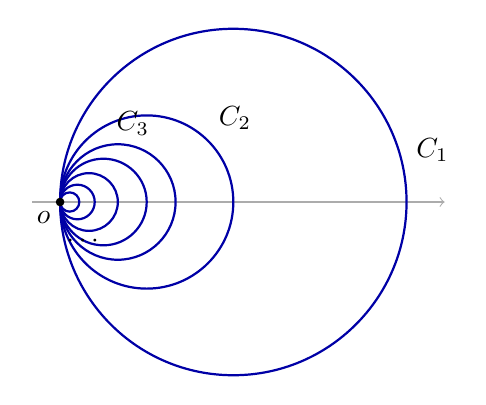
\begin{tikzpicture}[x=2.2cm,y=2.2cm]
	\draw[->,gray!65] (-0.16,0)--(2.22,0);
	\foreach \n in {1,2,3,4,6,10,18}{
		\pgfmathsetmacro{\rad}{1/\n}
		\draw[blue!65!black,thick] (\rad,0) circle[radius=\rad];
	}
	\fill (0,0) circle[radius=0.025];
	\node[below left] at (0,0) {\(o\)};
	\node[right] at (2,0.30) {\(C_1\)};
	\node[above right] at (0.86,0.36) {\(C_2\)};
	\node[above] at (0.42,0.33) {\(C_3\)};
	\node at (0.13,-0.23) {\(\cdots\)};
\end{tikzpicture}
% !TeX root = ../Book1.tex

		\caption{Hawaii 耳环中的若干圆周。图中只画出有限多个；完整空间含全部 \(C_n\)，它们都通过 \(o\)，且直径趋于零。任意小的 \(o\) 的邻域仍包含完整的小圆周。}
		\label{g1:fig:hawaiian-earring}
	\end{figure}

	固定 \(n\)，定义 \(r_n:Z\to C_n\)，在 \(C_n\) 上恒等，在其他圆周上恒取 \(o\)。它连续：在 \(o\) 处有 \(\|r_n(z)\|\le\|z\|\)；在非 \(o\) 点附近，可以避开所有其他圆周，或避开 \(C_n\)，因为足够小的圆周全都挤在 \(o\) 附近，而其余只有有限个。因而 \(r_n\) 是连续缩回。绕 \(C_n\) 一周的环路若在 \(Z\) 中零伦，复合 \(r_n\) 就会使它在 \(C_n\) 中零伦，这与\cref{g1:thm:circle-fundamental}矛盾。

	然而 \(o\) 的每个邻域都包含充分大的 \(n\) 对应的整个 \(C_n\)，因为 \(C_n\subseteq\overline B(o,2/n)\)。所以任意小邻域都有在 \(Z\) 中不能缩掉的环路，\(Z\) 不半局部单连通。

	若存在单连通覆盖 \(q:Y\to Z\)，取 \(o\) 的均匀覆盖邻域 \(U\) 及其上面任意一片。充分小的整个 \(C_n\) 位于 \(U\)；绕它一周的环路可经该片的局部逆提升为 \(Y\) 中的环路。它在单连通的 \(Y\) 中零伦，投影后便在 \(Z\) 中零伦，矛盾。因此 \(Z\) 不存在万有覆盖。这个论证只使用单个圆周的基本群，不需要描述 \(\pi_1(Z,o)\) 的全部结构。
\end{example}

在道路类构造中，失败发生在一个明确位置：如果邻域 \(U\) 中还有在 \(X\) 内非零伦的环路 \(\beta\)，则 \([\alpha]\) 与 \([\alpha*\beta]\) 有相同投影，却未必相同。因此 \(B([\alpha],U)\to U\) 可能不单射，也就不能作为覆盖的一片。

局部道路连通的职责则不同。\cref{g1:exm:topologist-sine}中的拓扑正弦曲线 \(S\) 在竖直线段上的道路分支不是开集，故没有道路连通开邻域基。取它的锥，可以保留局部道路连通性的障碍，同时使整个空间可缩：
\[
	C(S)=\{((1-t)x,(1-t)y,t):(x,y)\in S,\ 0\le t\le1\}\subseteq\mathbb R^3.
\]
顶点为 \(v=(0,0,1)\)。每个点都能沿直线连到 \(v\)，且直线同伦 \((z,s)\mapsto(1-s)z+sv\) 始终留在锥中，因此 \(C(S)\) 可缩，特别是道路连通、单连通并半局部单连通。不过在开集 \(V=\{t<1/2\}\cap C(S)\) 内，坐标变换
\[
	((1-t)x,(1-t)y,t)\longmapsto((x,y),t)
\]
给出 \(V\cong S\times[0,1/2)\)。点 \(((0,0),0)\) 的每个相对开邻域都遇到正弦图像上的点；若它有包含于 \(V\) 的道路连通开邻域，投影到 \(S\) 就会给出从竖直线段到正弦图像的道路，与\cref{g1:exm:topologist-sine}矛盾。因此这个单连通空间仍不局部道路连通。在它上面，恒等映射当然是万有覆盖，但上述“在任意给定邻域内取好邻域”的拓扑基论证不能照搬。

在道路类构造中，半局部单连通保证局部单射，局部道路连通保证好邻域构成原拓扑的基。锥的例子同时说明，特定空间即使缺少后一个条件，也可能有万有覆盖。关于本节道路类模型与覆盖分类的进一步阅读，可参见\cite[第1.3节]{Hatcher2002}。

% !TeX root = ../../Book1.tex
% 纲要标题：### 5.5 群作用、单值与覆盖的重建
% 纲要位置：几何学计划纲要.md，第 306 行。
% 正文状态：初稿；尚未正式审核。

% 纲要内容开始
% 
% * 适当不连续作用构造商覆盖
% * 纤维上的置换单值
% * 由单值数据重建覆盖
% * 环面、曲面及图覆盖的计算
% 
% ---
% 
% 纲要内容结束

\section{群作用、单值与覆盖的重建}
\label{g1:sec:0505}

沿底空间的道路行走时，覆盖中的起点一旦选定，整条提升就被确定了。如果底空间中的道路回到原点，提升却可能到达同一纤维的另一个点。于是环路给出纤维的一次置换。上一节用子群描述一个连通覆盖；本节把纤维的所有点一起保留，用这种置换记录整个覆盖，也允许覆盖不连通。

\subsection{适当不连续作用构造商覆盖}
\label{g1:subsec:0505:01}

第四章已经提醒，群轨道的商不一定是良好的几何空间：有理平移的商甚至只有平凡拓扑。要得到覆盖，所需条件相当具体：每一点应有一个小邻域，它的不同平移副本互不相交。这样，一个小邻域在取商时只被复制和识别，不会在内部折叠。

\begin{definition}[用于覆盖的适当不连续作用]\label{g1:def:properly-discontinuous-covering}
	设群 \(\Gamma\) 通过同胚左作用于拓扑空间 \(E\)。本节称该作用\term[shidangbulianxuzuoyong]{适当不连续}[properly discontinuous]，如果对每个 \(e\in E\)，都存在开邻域 \(V\ni e\)，使
	\[
		gV\cap V=\varnothing\qquad(g\in\Gamma,\ g\ne1).
	\]
	此约定包含自由性：若 \(ge=e\)，上述邻域立即迫使 \(g=1\)。有的文献允许非平凡点稳定子群而使用同一术语，应用其结论时需要核对定义。
\end{definition}

\begin{proposition}[作用的商是覆盖]\label{g1:prop:action-quotient-cover}
	设 \(\Gamma\) 在非空拓扑空间 \(E\) 上有上述作用，商集 \(E/\Gamma\) 取商拓扑。则轨道映射 \(q:E\rightarrow E/\Gamma\) 为覆盖。若 \(E\) 连通，则这个覆盖的甲板变换群恰为给定的 \(\Gamma\)；若 \(E\) 还单连通，则它是一个万有覆盖。
\end{proposition}
\begin{proof}
	对任意开集 \(O\subseteq E\)，有
	\[
		q^{-1}(q(O))=\bigcup_{g\in\Gamma}gO,
	\]
	右边开，故 \(q\) 为开映射。取定义中的 \(V\)。它的各个平移 \(gV\) 两两不交：若 \(gV\cap hV\ne\varnothing\)，则 \(h^{-1}gV\cap V\ne\varnothing\)，从而 \(g=h\)。由于 \(q|_V\) 连续、单射、开，且映满 \(q(V)\)，它为同胚；每个 \(q|_{gV}\) 同样为同胚。因此
	\[
		q^{-1}(q(V))=\bigsqcup_{g\in\Gamma}gV
	\]
	正是覆盖的局部形式。

	每个 \(g\) 保持轨道，故为甲板变换。反过来，若 \(E\) 连通且 \(T\) 是任意甲板变换，固定 \(e\in E\)，由同纤维就是同轨道，可找唯一 \(g\) 使 \(T(e)=ge\)。映射 \(T\) 与 \(g\) 都是 \(q\) 到自身的提升，由\cref{g1:prop:deck-determined}，在一点相等便处处相等。所以没有额外的甲板变换。单连通时，按万有覆盖的定义即得最后结论。
\end{proof}

整数群在 \(\mathbb R\) 上的平移满足此条件，因为长度小于 \(1\) 的开区间与其非零整数平移不交。由 \(t\mapsto e^{2\pi it}\) 可识别 \(\mathbb R/\mathbb Z\cong S^1\)，得到圆周的万有覆盖。反之，\(\mathbb Q\) 的平移在任何开区间中都有非零的小平移与自身相交，恰好失去这一条件。反射 \(x\mapsto-x\) 的作用在原点有稳定子群，其商映射 \(\mathbb R\rightarrow[0,\infty)\) 在原点附近也不是覆盖：任一含原点的开区间都包含两个被识别的点，不能成为一张同胚覆盖片。

\begin{proposition}[万有覆盖上的基本群作用]\label{g1:prop:universal-deck-discontinuous}
	设 \(X\) 非空、道路连通、局部道路连通且半局部单连通，\(\widetilde X\) 是从基点 \(x_0\) 出发的道路类万有覆盖，\(G=\pi_1(X,x_0)\)。由
	\[
		L_g[\alpha]=[\gamma*\alpha]\qquad(g=[\gamma])
	\]
	给出的 \(G\) 左作用适当不连续，而且在每个纤维上自由且传递。
\end{proposition}
\begin{proof}
	这些映射及其群乘法由\cref{g1:thm:normal-covering-deck}给出。若道路 \(\alpha,\beta\) 终点相同，取 \(g=[\beta*\bar\alpha]\)，便有 \(L_g[\alpha]=[\beta]\)，故作用在纤维上传递；自由性来自甲板变换由一点决定。

	取底空间一个连通的均匀覆盖邻域 \(U\)，并取上方一张片 \(V\)。每个 \(L_g\) 把 \(V\) 映到 \(U\) 上方的一张片，因为它保持投影，且片可由道路提升从其中一点得到。若 \(L_gV\) 与 \(V\) 相交，两片必相同。此时投影在 \(V\) 上单射，迫使 \(L_g|_V=\operatorname{id}_V\)，再由甲板变换的确定性得到 \(g=1\)。因此 \(V\) 的不同群平移两两不交。
\end{proof}

这里的“均匀覆盖邻域”指其原像分解成同胚覆盖片的开邻域；连通的选择由底空间局部道路连通保证。它与前一节道路类构造中的好邻域是同一类局部工具。

\subsection{纤维上的置换单值}
\label{g1:subsec:0505:02}

现在固定任意覆盖 \(p:E\rightarrow X\) 和基点 \(x_0\in X\)，令 \(S=p^{-1}(x_0)\)。这一纤维是离散空间，但其点不需要预先排列成编号。我们把“从哪一点出发，沿环路以后到哪一点”作为置换的定义。

\begin{proposition}[单值的右作用]\label{g1:prop:monodromy-action}
	设 \(p:E\rightarrow X\) 为覆盖，\(x_0\in X\)，\(G=\pi_1(X,x_0)\)。对 \(s\in S=p^{-1}(x_0)\) 与 \(g=[\gamma]\in G\)，定义
	\[
		s\cdot g=\widetilde\gamma_s(1),
	\]
	其中 \(\widetilde\gamma_s\) 是从 \(s\) 出发的唯一道路提升。则此公式良定义，并构成 \(G\) 在 \(S\) 上的右作用。这称为覆盖的\term[danzhizuoyong]{单值作用}[monodromy action]。
\end{proposition}
\begin{proof}
	\cref{g1:cor:lifted-path-homotopy}保证同伦的环路从同一纤维点提升后有相同终点，所以结果只依赖 \(g\)。常值道路的提升常值，故 \(s\cdot1=s\)。先走 \(\gamma\) 再走 \(\eta\) 时，可以先提升 \(\gamma\)，再从其终点提升 \(\eta\)；两段拼接是 \(\gamma*\eta\) 的提升，由唯一性就是全部提升。因此
	\[
		(s\cdot g)\cdot h=s\cdot(gh).
	\]
	沿反路提升把终点送回起点，所以每个 \(g\) 给出的映射均为置换，逆置换由 \(g^{-1}\) 给出。
\end{proof}

本书先走左边道路的乘法约定，自然产生右作用。若把 \(s\mapsto s\cdot g\) 记作置换 \(M_g\)，并按通常函数复合记乘法，则 \(M_{gh}=M_h\circ M_g\)。若希望得到按通常复合的群同态 \(G\rightarrow\operatorname{Sym}(S)\)，应取 \(g\mapsto M_{g^{-1}}\)。后面直接使用右作用等式，避免在两个约定之间来回转换。

\begin{proposition}[轨道、稳定子群与覆盖的连通性]\label{g1:prop:monodromy-components}
	设 \(X\) 非空、道路连通且局部道路连通，\(p:E\rightarrow X\) 为覆盖，\(S=p^{-1}(x_0)\)。
	\begin{enumerate}
		\item \(S\) 的单值轨道与 \(E\) 的连通分支一一对应。因此 \(E\) 连通当且仅当单值作用传递。
		\item 对 \(s\in S\)，其稳定子群是 \(p_*\pi_1(E,s)\subseteq G\)。
		\item 设该子群为 \(H\)。轨道 \(sG\) 与陪集集合 \(H\backslash G=\{Hg:g\in G\}\) 右等变双射，对应为 \(Hg\mapsto s\cdot g\)。
	\end{enumerate}
\end{proposition}
\begin{proof}
	由覆盖的局部形式，\(E\) 局部道路连通，故由\cref{g1:thm:locally-path-components}，连通分支就是道路分支。每个分支都遇到 \(S\)：从任一点的投影沿道路到 \(x_0\)，提升后就在同一分支中到达 \(S\)。两点 \(s,t\in S\) 能在 \(E\) 中用道路相连，当且仅当某个底空间环路的提升从 \(s\) 到 \(t\)，这正是二者属于同一单值轨道，得到第一项。

	等式 \(s\cdot g=s\) 意味着对应提升是闭路；由\cref{g1:cor:closed-lift-criterion}，这恰好等价于 \(g\in p_*\pi_1(E,s)\)，得到第二项。最后，
	\[
		s\cdot g=s\cdot h
		\quad\Longleftrightarrow\quad gh^{-1}\in H
		\quad\Longleftrightarrow\quad Hg=Hh.
	\]
	故陪集对应良定义且单射，满射由轨道的定义得到；右乘的相容性也直接来自作用等式。
\end{proof}

例如 \(z\mapsto z^n\)（\(n\ge1\)）的纤维可标为 \(s_j=e^{2\pi ij/n}\)，\(j\in\mathbb Z/n\mathbb Z\)。一周正向环路从 \(s_j\) 提升为 \(e^{2\pi i(t+j)/n}\)，终点是 \(s_{j+1}\)。所以基本群的生成元在纤维上作一个 \(n\)-循环，其稳定子群为 \(n\mathbb Z\)。一个局部选出的 \(n\) 次根沿圆周继续一周以后会改变分支，这就是单值作用所记录的现象。

\subsection{由单值数据重建覆盖}
\label{g1:subsec:0505:03}

反过来，若只给一个集合 \(S\)，以及底空间环路如何置换 \(S\) 的规则，能否找回覆盖？万有覆盖已经把每条道路的行走历史保存为道路类；把历史改变时纤维编号应如何改变一并规定，就能作出所需商空间。

\begin{theorem}[由右群作用重建覆盖]\label{g1:thm:monodromy-reconstruction}
	设 \(X\) 非空、道路连通、局部道路连通且半局部单连通，固定 \(x_0\)，令 \(G=\pi_1(X,x_0)\)，\(\widetilde p:\widetilde X\rightarrow X\) 为道路类万有覆盖。对任意非空右 \(G\) 集合 \(S\)，赋予 \(S\) 离散拓扑，并在 \(S\times\widetilde X\) 上定义左作用
	\[
		g\cdot(s,u)=(s\cdot g^{-1},L_g u).
	\]
	则轨道商
	\[
		E_S=(S\times\widetilde X)/G,\qquad p_S([s,u])=\widetilde p(u)
	\]
	是 \(X\) 上的覆盖。其基点纤维自然等于 \(S\)，单值作用就是原给定右作用。每个非空覆盖均由此得到，两个这样的覆盖同构当且仅当其纤维右 \(G\) 集合同构。
\end{theorem}
\begin{proof}
	先核验群作用方向。连续施以 \(h\) 再施以 \(g\)，第一坐标变为 \(s\cdot h^{-1}g^{-1}=s\cdot(gh)^{-1}\)，第二坐标变为 \(L_{gh}u\)，所以确为左作用。每个作用映射为同胚，且保持 \(\widetilde p(u)\)，因此 \(p_S\) 良定义且连续。商映射 \(q:S\times\widetilde X\rightarrow E_S\) 开，证明与\cref{g1:prop:action-quotient-cover}相同。

	取连通的均匀覆盖邻域 \(U\subseteq X\) 和万有覆盖的一张片 \(V\)。由\cref{g1:prop:universal-deck-discontinuous}，其他各片恰为 \(L_gV\)，而且指标 \(g\) 唯一。对每个 \(s\in S\)，令 \(W_s=q(\{s\}\times V)\)。这些集合开，并且 \(q\) 将 \(\{s\}\times V\) 同胚地映到 \(W_s\)：若其中两点被识别，则某个 \(L_gV\) 与 \(V\) 相交，迫使 \(g=1\)。同样的论证说明不同 \(s\) 给出的 \(W_s\) 不交。若 \(u=L_gv\)、\(v\in V\)，轨道关系给出
	\begin{equation}\label{g1:eq:associated-cover-relation}
		[s,L_gv]=[s\cdot g,v],
	\end{equation}
	所以这些 \(W_s\) 覆盖 \(p_S^{-1}(U)\)，且每个 \(p_S|_{W_s}\) 与 \(\widetilde p|_V\) 对应，为到 \(U\) 的同胚。这证明覆盖性质。

	记万有覆盖基点为 \(\widetilde x_0=[e_{x_0}]\)。纤维点写成 \([s,\widetilde x_0]\) 的方式唯一，故基点纤维与 \(S\) 相同。从此点提升代表 \(g\) 的环路 \(\gamma\)，可以使用道路 \(t\mapsto[s,\widetilde\gamma(t)]\)，其中 \(\widetilde\gamma\) 从 \(\widetilde x_0\) 出发。其终点为
	\[
		[s,L_g\widetilde x_0]=[s\cdot g,\widetilde x_0],
	\]
	所以单值恰为指定的右作用。

	再设 \(p:E\rightarrow X\) 是任意覆盖，\(S=p^{-1}(x_0)\) 取其单值作用。对每个 \(s\)，由\cref{g1:thm:lifting-criterion}，\(\widetilde p\) 有唯一连续提升 \(F_s:\widetilde X\rightarrow E\) 满足 \(F_s(\widetilde x_0)=s\)：定义域道路连通、局部道路连通且单连通，因此基本群包含条件自动成立。具体地，\(F_s([\alpha])\) 是 \(\alpha\) 从 \(s\) 出发的提升终点。映射 \(F(s,u)=F_s(u)\) 在离散积上连续。先从 \(s\cdot g^{-1}\) 提升 \(\gamma\)，会回到 \(s\)，然后提升 \(\alpha\)，故
	\[
		F(s\cdot g^{-1},L_g[\alpha])=F(s,[\alpha]).
	\]
	它因而下降为连续映射 \(\bar F:E_S\rightarrow E\)，并保持到底空间的投影。

	给定 \(x\in X\) 及一条从 \(x_0\) 到 \(x\) 的道路 \(\alpha\)，沿 \(\alpha\) 提升给出纤维 \(S\rightarrow p^{-1}(x)\) 的双射，其逆由反路提升给出。另一方面，\(E_S\) 中 \(x\) 上方的点也唯一写成 \([s,[\alpha]]\)。所以 \(\bar F\) 在每个纤维上双射，因而全局双射。它在足够小的共同均匀覆盖邻域上逐片等于两张同胚片之间的坐标对应，故为局部同胚；双射局部同胚是同胚。因此找回了原覆盖。

	最后，覆盖同构限制到基点纤维后与道路提升相容，故是右 \(G\) 集合的同构。反过来，右等变双射 \(\phi:S\rightarrow S'\) 使 \((s,u)\mapsto(\phi(s),u)\) 与轨道关系相容，下降为 \(E_S\rightarrow E_{S'}\) 的同构，逆映射由 \(\phi^{-1}\) 给出。
\end{proof}

若允许空总空间，空集合也对应一个空的局部覆盖；本章覆盖按满射定义，所以定理明确使用非空 \(S\)。在连通情形，传递右 \(G\) 集合写成 \(H\backslash G\)，便恢复上一节的子群分类。这里的重建还保留了不同轨道，因此同时处理不连通覆盖。

\begin{corollary}[甲板变换与等变置换]\label{g1:cor:deck-centralizer}
	在上一定理的假设下，任一覆盖 \(E\rightarrow X\) 的甲板变换群，等于其纤维 \(S\) 上与全部单值置换交换的置换群。
\end{corollary}
\begin{proof}
	甲板变换将从 \(s\) 出发的道路提升送到从 \(T(s)\) 出发的提升，因此 \(T(s\cdot g)=T(s)\cdot g\)。反过来，每个满足此等式的纤维置换由定理的重建公式扩张为甲板变换。扩张唯一：每一点都是某条从基点纤维出发的提升道路的终点，而该终点的像已由纤维置换决定。限制与扩张保持函数复合，所以给出群同构。
\end{proof}

单值作用和甲板变换作用因此不是同一件事。前者由底空间环路推动纤维点，后者是整个覆盖保持投影的对称；后者必须与前者交换。

\subsection{环面、曲面及图覆盖的计算}
\label{g1:subsec:0505:04}

先看环面。由\cref{g1:prop:product-fundamental}，\(\pi_1(T^2)\cong\mathbb Z^2\)，而逐坐标指数映射
\[
	P:\mathbb R^2\longrightarrow T^2,\qquad P(u,v)=(e^{2\pi iu},e^{2\pi iv})
\]
为万有覆盖：两个圆周覆盖片的积给出覆盖局部形式，\(\mathbb R^2\) 凸而单连通。甲板群是整数平移。对子群 \(H\le\mathbb Z^2\)，得到连通覆盖 \(\mathbb R^2/H\rightarrow T^2\)，纤维为 \(H\backslash\mathbb Z^2\)。因为底群交换，这些连通覆盖全部正规。

\begin{example}[一个六叶环面覆盖]\label{g1:exm:torus-six-cover}
	取 \(H=\langle(2,0),(1,3)\rangle\)。线性映射 \(A(u,v)=(2u+v,3v)\) 将 \(\mathbb Z^2\) 映到 \(H\)，并诱导同胚 \(\mathbb R^2/\mathbb Z^2\rightarrow\mathbb R^2/H\)。所以相应覆盖可写成
	\[
		f:T^2\longrightarrow T^2,\qquad f(z,w)=(z^2w,w^3).
	\]
	每个陪集都有唯一代表 \((r,s)\)，其中 \(r=0,1\)，\(s=0,1,2\)：先用 \((1,3)\) 把第二坐标约化到这三个值，再用 \((2,0)\) 约化第一坐标；若两个代表之差在 \(H\)，第二坐标差迫使 \((1,3)\) 的系数为零，再由第一坐标得到两代表相同。因此叶数为 \(6\)。

	令 \(e_1=(1,0),e_2=(0,1)\)。商群中 \(2e_1=0\)、\(e_1+3e_2=0\)，所以 \(e_1=-3e_2\)，全群由 \(e_2\) 生成且有六个元素，即甲板群为 \(\mathbb Z/6\mathbb Z\)。沿两个圆周生成环路的单值分别是陪集加 \(e_1,e_2\)，在这一循环编号下分别为加 \(3\)、加 \(1\)。这同时给出了覆盖公式、叶数、单值与甲板群。
\end{example}

对由标准边字
\[
	[a_1,b_1]\cdots[a_g,b_g],\qquad [a,b]=aba^{-1}b^{-1},
\]
得到的可定向多边形曲面模型 \(\Sigma_g\)，先对其 \(2g\) 条边组成的一点并图使用\cref{g1:prop:graph-fundamental}，再由\cref{g1:prop:attach-disk}沿该边字附着圆盘，就得到以这些生成元和该关系为展示的基本群（\(g\ge1\)）。构造 \(n\) 叶覆盖时，可在 \(S=\{1,\ldots,n\}\) 上指定各生成元的右置换；唯一需要检查的关系是按该边字依次作用后恒等。这保证自由群作用通过所展示的商群下降，再由\cref{g1:thm:monodromy-reconstruction}得到覆盖。生成置换的轨道决定覆盖的连通分支。这里使用的是明确的多边形模型及其关系，不需要预先知道所有紧曲面的分类。

例如 \(g\ge1\) 时，令 \(a_1\) 作 \(n\)-循环，其余 \(a_i,b_i\) 全部恒等。每个交换子作用都恒等，所以关系满足；\(n\)-循环使作用传递，故得到连通 \(n\) 叶覆盖。单值通过满同态 \(\pi_1(\Sigma_g)\rightarrow\mathbb Z/n\mathbb Z\) 的正则作用给出，稳定子群就是该同态的核，因而此覆盖正规，甲板群为 \(\mathbb Z/n\mathbb Z\)。

\begin{example}[图覆盖中单值与甲板群的差别]\label{g1:exm:three-sheet-graph}
	设 \(B\) 为两个圆周 \(a,b\) 在一点相接的图，\(\pi_1(B)=F(a,b)\)。在三个纤维点上规定右置换
	\[
		s\cdot a=(12)(s),\qquad s\cdot b=(23)(s).
	\]
	自由群没有关系，故这给出一个右作用：一个字从左到右逐个作用即可。构造覆盖图时，在顶点 \(1,2,3\) 之间，为每个 \(s\) 放一条从 \(s\) 到 \(s\cdot a\) 的有向 \(a\)-边，再放一条从 \(s\) 到 \(s\cdot b\) 的有向 \(b\)-边。每条边按参数同胚地映到基图相应边的内部。

	在每个顶点附近，各有一条 \(a\)-边进入、一条 \(a\)-边离开，以及对应的两条 \(b\)-半边；环边也分别贡献进入、离开的半边。因此顶点的小星形邻域同胚地映到基图基点的小星形邻域，边内部也显然满足覆盖条件，得到三叶图覆盖。两次换位生成传递作用，所以覆盖连通。图有三个顶点和六条边，由\cref{g1:prop:graph-fundamental}，其基本群为秩 \(6-3+1=4\) 的自由群。

	单值置换生成 \(S_3\)，但甲板群平凡。事实上，若置换 \(T\) 同时与 \((12)\)、\((23)\) 交换，它必须分别保留二者唯一的不动点 \(3,1\)，于是也固定 \(2\)，所以 \(T=\operatorname{id}\)。由\cref{g1:cor:deck-centralizer}，覆盖没有非平凡甲板变换。覆盖连通只说明单值传递，并不保证甲板变换能把任意纤维点送到另一个。
\end{example}

\begin{figure}[htbp]
	\centering
	% !TeX root = ../Book1.tex
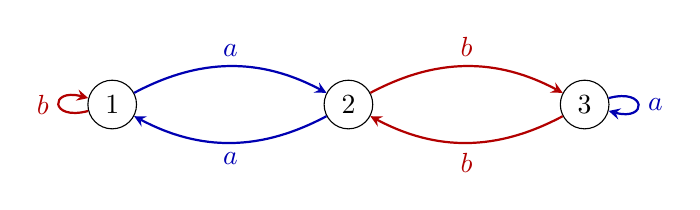
\begin{tikzpicture}[x=1cm,y=1cm,>=stealth]
	\node[circle,draw,minimum size=6mm] (v1) at (0,0) {\(1\)};
	\node[circle,draw,minimum size=6mm] (v2) at (3,0) {\(2\)};
	\node[circle,draw,minimum size=6mm] (v3) at (6,0) {\(3\)};
	\draw[blue!70!black,thick,->] (v1) to[bend left=28] node[above] {\(a\)} (v2);
	\draw[blue!70!black,thick,->] (v2) to[bend left=28] node[below] {\(a\)} (v1);
	\draw[red!70!black,thick,->] (v2) to[bend left=28] node[above] {\(b\)} (v3);
	\draw[red!70!black,thick,->] (v3) to[bend left=28] node[below] {\(b\)} (v2);
	\draw[red!70!black,thick,->] (v1) to[loop left] node[left] {\(b\)} (v1);
	\draw[blue!70!black,thick,->] (v3) to[loop right] node[right] {\(a\)} (v3);
\end{tikzpicture}

	\caption{二圈图的三叶覆盖。蓝色边标记 \(a\)，红色边标记 \(b\)；同一对顶点间的两条反向边是两条不同的边。每个顶点都有各标记的一入一出，纤维置换分别为 \((12)\) 与 \((23)\)。}
	\label{g1:fig:three-sheet-graph}
\end{figure}

这些例子显示两种计算可以相互检查。先从图形或粘合求基本群，再用它在纤维上的作用建立覆盖；反过来，提升终点、叶数和甲板变换又能检验原来的群与关系。关于覆盖、群作用和图的进一步阅读，可参阅\cite[Section 1.3; Section 1.A]{Hatcher2002}。


\begin{chaptersummary}
	定端点同伦允许改变道路的形状与速度，但保留起终点。环路类的拼接给出基本群，连续映射诱导群同态；沿道路改变基点得到同构，不同选择之间相差内自同构。形变收缩保留基本群，圆周角度的提升把基本群识别为整数绕数，积空间的基本群则逐坐标计算。

	\ProseParagraphBreak

	van Kampen 定理将粘合转成自由积与关系。细分道路给出生成元，细分同伦方形说明全部关系由交集中的环路产生。有限连通图的生成元来自生成树之外的边，附着圆盘将边界词的正规闭包消去；这种计算同时解释了图、去点空间和曲面模型中环路为何保留或消失。

	\ProseParagraphBreak

	覆盖的均匀局部结构使道路逐段唯一提升，同伦提升保证终点只依赖道路类。覆盖在基本群上诱导单射，一个映射能否提升由其基本群像是否落入覆盖子群判断。覆盖变换由一个点的像决定，需要总空间连通；它反映整个覆盖的对称，而不能仅从纤维点数推断。

	\ProseParagraphBreak

	道路类构造把“到达同一点的不同历史”保留下来。局部道路连通提供适用的道路邻域，半局部单连通保证小环路在全空间内零伦，从而让终点映射在基本邻域上单射。带基点连通覆盖对应基本群子群，忘掉基点对应共轭类，正规覆盖对应正规子群；一般覆盖变换群为 \(N_G(H)/H\)，正规时才是 \(G/H\)。

	\ProseParagraphBreak

	沿环路提升使基本群右作用于纤维，轨道给出覆盖的连通分支，稳定子给出相应子群。反过来，把这个右作用与万有覆盖的左覆盖变换作用配对取商，就能重建覆盖。覆盖变换群由与全部单值置换交换的置换组成；环面和图的计算说明，单值传递、覆盖正规以及覆盖变换群传递必须分别判断。
\end{chaptersummary}

\BookExercises
以下各题均给出完整解答。计算基本群时注明基点及所用粘合条件；构造覆盖时检查局部拓扑，并区分单值作用、子群与覆盖变换。

\begin{exercise}\label{g1:ex:loop-disk-extension}
	设 \(f:S^1\rightarrow X\) 连续，\(x_0=f(1)\)，并令 \(\alpha(t)=f(e^{2\pi it})\)。证明 \([\alpha]=1\in\pi_1(X,x_0)\)，当且仅当 \(f\) 可以连续延拓为 \(F:D^2\rightarrow X\)，其中 \(D^2=\{z\in\mathbb C:|z|\le1\}\)。
\end{exercise}
\begin{solution}
	若 \(H(t,u)\) 是把 \(\alpha\) 固定端点收缩到 \(x_0\) 的同伦，定义
	\[
		F(re^{2\pi it})=H(t,1-r)\qquad(0\le r\le1).
	\]
	当 \(r=0\) 时右边恒为 \(x_0\)，当 \(t=0,1\) 时两式也都为 \(x_0\)，所以选择极角无关。为验证圆心处的连续性而不依赖极坐标直觉，使用连续满射 \(q:[0,1]^2\rightarrow D^2\)、\(q(t,r)=re^{2\pi it}\)。定义域紧、目标 Hausdorff，所以 \(q\) 闭，从而是商映射。连续函数 \((t,r)\mapsto H(t,1-r)\) 在它的每个纤维上常值，故由商下降得到连续 \(F\)。边界 \(r=1\) 处的值正是 \(f\)。

	反之，若 \(F\) 存在，取
	\[
		H(t,u)=F\bigl((1-u)e^{2\pi it}+u\bigr).
	\]
	单位圆盘凸，括号中的点始终在圆盘内。\(u=0\) 时得到 \(\alpha\)，\(u=1\) 时恒为 \(F(1)=x_0\)；\(t=0,1\) 时括号中都为 \(1\)，所以两端固定。这就是所需同伦。
\end{solution}

\begin{exercise}\label{g1:ex:no-disk-boundary-retraction}
	证明不存在连续映射 \(r:D^2\rightarrow S^1\) 满足 \(r|_{S^1}=\operatorname{id}_{S^1}\)。为什么这不妨碍穿孔圆盘向边界作径向形变收缩？
\end{exercise}
\begin{solution}
	若存在，包含映射 \(i:S^1\hookrightarrow D^2\) 满足 \(r\circ i=\operatorname{id}\)，所以 \(r_*i_*=\operatorname{id}_{\mathbb Z}\)。然而圆盘凸，基本群平凡，故 \(i_*\) 的像为零，复合 \(r_*i_*\) 也只能是零同态，与 \(\mathbb Z\) 的恒等同态不同。因此缩回不存在。

	穿孔圆盘 \(\{0<|z|\le1\}\) 上 \(r(z)=z/|z|\) 连续，且
	\[
		H(z,u)=\left(1-u+\frac{u}{|z|}\right)z
	\]
	的模为 \((1-u)|z|+u\in(0,1]\)，故始终留在穿孔圆盘内，并固定边界。这个公式在 \(z=0\) 无定义，不能连续补上；正是删去圆心改变了基本群。
\end{solution}

\begin{exercise}\label{g1:ex:topological-group-pi1-abelian}
	设 \(K\) 是拓扑群，单位元为 \(e\)；这里群乘法 \(K\times K\rightarrow K\) 和取逆都连续。证明 \(\pi_1(K,e)\) 为交换群，不要求 \(K\) 本身交换。
\end{exercise}
\begin{solution}
	取两个基于 \(e\) 的环路 \(\alpha,\beta\)，考虑方形映射 \(F(s,t)=\alpha(s)\beta(t)\)。沿下边再右边从 \((0,0)\) 到 \((1,1)\)，其像是 \(\alpha*\beta\)；沿左边再上边，其像是 \(\beta*\alpha\)，因为 \(\alpha,\beta\) 在端点都取 \(e\)。这两条方形内的折线路径可以定端点线性插值，插值仍留在凸方形中。与 \(F\) 复合，就给出 \(\alpha*\beta\simeq\beta*\alpha\) 的定端点同伦。所以任意两个基本群元素交换。整个证明没有交换 \(K\) 中两个任意元素，只比较了方形边界上因端点取单位元而简化的乘积。
\end{solution}

\begin{exercise}\label{g1:ex:torus-induced-matrix}
	对映射 \(f:T^2\rightarrow T^2\)、\(f(z,w)=(z^2w^{-1},z^3w^2)\)，在两个坐标圆周环路给出的 \(\pi_1(T^2,(1,1))\cong\mathbb Z^2\) 下求 \(f_*\)。证明 \(f\) 不是同胚，也不与常值映射同伦。
\end{exercise}
\begin{solution}
	第一生成环路 \(a(t)=(e^{2\pi it},1)\) 的像绕数为 \((2,3)\)，第二生成环路 \(b(t)=(1,e^{2\pi it})\) 的像绕数为 \((-1,2)\)。所以
	\[
		f_*\binom{m}{n}
		=\begin{pmatrix}2&-1\\3&2\end{pmatrix}\binom{m}{n}
		=\binom{2m-n}{3m+2n}.
	\]
	它不满射：若像为 \((1,0)\)，由 \(n=2m-1\) 得 \(7m=2\)，没有整数解。同胚必须诱导群同构，故 \(f\) 不是同胚。若 \(f\) 与常值映射同伦，基点可能在同伦中移动，但\cref{g1:prop:moving-basepoint}说明相应诱导同态只相差一个基点变化同构。常值映射的诱导同态为零，于是 \(f_*\) 也须为零，与 \(f_*(1,0)=(2,3)\) 矛盾。
\end{solution}

\begin{exercise}\label{g1:ex:radial-winding}
	在 \(\mathbb C\setminus\{0\}\) 中考虑从 \(3\) 出发并回到 \(3\) 的环路
	\[
		\gamma(t)=(2+\cos2\pi t)e^{4\pi it}.
	\]
	求它经径向缩回到圆周后的绕数，写出与两周标准圆周环路之间的自由同伦（中间各曲线仍为环路，但基点允许移动），并说明该同伦为什么不是原基点 \(3\) 处的定端点同伦。
\end{exercise}
\begin{solution}
	因为 \(2+\cos2\pi t\ge1\)，\(\gamma\) 从不为零，其径向缩回为 \(e^{4\pi it}\)，连续角度为 \(2t\)，所以绕数为 \(2\)。公式
	\[
		H(t,u)=\bigl((1-u)(2+\cos2\pi t)+u\bigr)e^{4\pi it}
	\]
	给出连续同伦，每个 \(u\) 处都是环路，且系数始终正。在 \(t=0,1\) 处，它的值为 \(3-2u\)，从 \(3\) 移动到 \(1\)，所以端点虽彼此相同却没有固定不动。若要在基点 \(3\) 处比较基本群元素，应把圆周环路与从 \(3\) 到 \(1\) 的径向道路及其反路拼接，使用\cref{g1:prop:basepoint-change}，不能把不同基点的两个环路直接认作同一基本群中的元素。
\end{solution}

\begin{exercise}\label{g1:ex:free-product-orders}
	设 \(G=\langle a,b\mid a^2=1,\ b^3=1\rangle\)。证明 \(G\cong(\mathbb Z/2\mathbb Z)*(\mathbb Z/3\mathbb Z)\)，证明 \(ab\) 有无限阶，并判断 \(aba^{-1}b^{-1}\) 是否为单位元。
\end{exercise}
\begin{solution}
	把 \(a\) 送到第一循环因子的生成元，把 \(b\) 送到第二循环因子的生成元，两个关系都成立，故群展示的泛性质给出到自由积的同态。反方向，由 \(a^2=1,b^3=1\)，两个循环群分别同态地映入 \(G\)，自由积的泛性质给出反向同态。两个复合在 \(a,b\) 上恒等，故在它们生成的群上恒等，得到所述同构。

	在自由积中，正整数 \(k\) 对应的词 \((ab)^k\) 有 \(2k\) 个非单位字母，相邻字母分属两个不同因子，故已经约化且不是空词。因此 \((ab)^k\ne1\)，\(ab\) 有无限阶。又 \(a^{-1}=a\)、\(b^{-1}=b^2\)，所以交换子为 \(abab^2\)。它同样是长度 \(4\) 的约化词，故不是单位元。两个生成元各自有有限阶，并不使自由积有限，也不使它们交换。
\end{solution}

\begin{exercise}\label{g1:ex:cube-graph}
	设 \(G\) 为立方体的顶点与棱组成的图，不包括任何面。计算 \(\pi_1(G)\)。若删去任一条棱的内部，所得图 \(G'\) 的基本群是什么？若改为把整张立方体表面加入 \(G\)，基本群又是什么？说明后两种操作为何不能混为一谈。
\end{exercise}
\begin{solution}
	立方体有 \(8\) 个顶点和 \(12\) 条棱，且图连通，故\cref{g1:prop:graph-fundamental}给出 \(\pi_1(G)\cong F_{12-8+1}=F_5\)。删去任一条棱的内部后，其两端仍可沿包含它的一个正方形面的其余三条棱连接；原先经过所删棱的任何边路都可用这三条棱替换，因此图仍连通。它有 \(11\) 条边、\(8\) 个顶点，故 \(\pi_1(G')\cong F_4\)。

	加入所有面所得空间同胚于 \(S^2\)。若立方体以原点为中心，边长为 \(2\)，由球面到其边界的同胚为
	\[
		u\longmapsto\frac{u}{\lVert u\rVert_\infty},\qquad
		\lVert u\rVert_\infty=\max\{|u_1|,|u_2|,|u_3|\},
	\]
	逆映射为 \(x\mapsto x/\lVert x\rVert\)，两个分母在各自空间中都不为零。正文已通过南北极开覆盖证明 \(\pi_1(S^2)=1\)，所以立方体表面的基本群平凡。删边减少可走的路线；添面保留原来的路线，却提供新的同伦把某些环路消去。这两种空间变化的机制不同，基本群的计算也不同。
\end{solution}

\begin{exercise}\label{g1:ex:degree-disk-attachment}
	对整数 \(m\)，将一个圆盘沿 \(f_m:S^1\to S^1,\ z\mapsto z^m\) 附着到一个圆周上，所得空间记为 \(X_m\)；当 \(m=0\) 时，\(f_0\) 为常值映射。计算 \(\pi_1(X_m)\)，并说明附着圆盘的包含关系为何不保证原圆周的基本群仍嵌入。
\end{exercise}
\begin{solution}
	取圆周上的基点 \(1\)，正向生成元为 \(a\)。沿圆盘边界走一周时，像环路为 \(t\mapsto e^{2\pi imt}\)，其绕数为 \(m\)，故代表 \(a^m\)。附着命题给出
	\[
		\pi_1(X_m)\cong\langle a\mid a^m=1\rangle
		\cong
		\begin{cases}
			\mathbb Z,&m=0,\\
			\mathbb Z/|m|\mathbb Z,&m\ne0.
		\end{cases}
	\]
	当 \(m=0\) 时，关系词已经是单位元，未添加新关系；当 \(m\ne0\) 时，包含映射在基本群上是 \(\mathbb Z\to\mathbb Z/|m|\mathbb Z\)，核为 \(m\mathbb Z\)，不是单射。空间中的点并未因为附着而把原圆周的不同点额外识别，但新增的圆盘允许原圆周中的环路在更大的空间内变形；点之间的映射是否单射，与同伦类之间的映射是否单射，是不同的问题。
\end{solution}

\begin{exercise}\label{g1:ex:puncture-commutator}
	取 \(X=\mathbb R^2\setminus\{p,q\}\)，按正文的去点空间构造选择自由生成元 \(a,b\)，分别绕 \(p,q\) 一周。证明环路类 \(aba^{-1}b^{-1}\) 非平凡，但它在两个包含映射
	\[
		X\hookrightarrow\mathbb R^2\setminus\{p\},\qquad
		X\hookrightarrow\mathbb R^2\setminus\{q\}
	\]
	诱导的同态下都变为单位元。说明这给“用每个缺失点的绕数判断是否可收缩”带来什么限制。
\end{exercise}
\begin{solution}
	\(\pi_1(X)\cong F(\{a,b\})\)，其中 \(aba^{-1}b^{-1}\) 没有任何相邻的逆字母，因而是长度 \(4\) 的非空约化词，不是单位元。

	在只去掉 \(p\) 的空间中，绕 \(q\) 的小圆周可以在不遇到 \(p\) 的小圆盘内收缩；接到基点的道路仅产生共轭，所以 \(b\) 的像为单位元。\(a\) 的像是该单点补空间的正向生成元，整个词的像遂为 \(a\cdot1\cdot a^{-1}\cdot1=1\)。另一个包含映射下 \(a\) 的像为单位元、\(b\) 为生成元，同样得到 \(1\)。

	因此这条环路对每个缺失点的整数绕数都为零，却不能在同时避开两点的空间中收缩。两个绕数只记录两个字母各自的指数和，会丢失先后次序。它们构成到 \(\mathbb Z^2\) 的同态，但不是对非交换自由群元素的完全判别。
\end{solution}

\begin{exercise}\label{g1:ex:torus-slope-attachment}
	取整数 \(p,q\)，沿环路 \(t\mapsto(e^{2\pi ipt},e^{2\pi iqt})\) 向环面 \(T^2\) 附着一张圆盘，所得空间为 \(Y_{p,q}\)。计算其基本群。对 \((p,q)\ne(0,0)\)，令 \(d=\gcd(|p|,|q|)\)，证明结果为 \(\mathbb Z\oplus\mathbb Z/d\mathbb Z\)。
\end{exercise}
\begin{solution}
	环面的生成元 \(a,b\) 交换，所给环路在积空间基本群中的坐标为 \((p,q)\)，亦即元素 \(a^pb^q\)。附着命题给出
	\[
		\pi_1(Y_{p,q})\cong
		\langle a,b\mid aba^{-1}b^{-1}=1,\ a^pb^q=1\rangle
		\cong\mathbb Z^2/\mathbb Z(p,q).
	\]
	若 \(p=q=0\)，所商子群为零，结果为 \(\mathbb Z^2\)。

	若 \((p,q)\ne(0,0)\)，取整数 \(r,s\) 使 \(rp+sq=d\)。这是最大公因数的整系数表示，可由辗转相除逐步回代求得。矩阵
	\[
		A=\begin{pmatrix}r&s\\-q/d&p/d\end{pmatrix}
	\]
	的行列式为 \(1\)，其逆矩阵仍有整数条目，故给出 \(\mathbb Z^2\) 的自同构；同时 \(A(p,q)^{\mathsf T}=(d,0)^{\mathsf T}\)。于是
	\[
		\mathbb Z^2/\mathbb Z(p,q)
		\cong\mathbb Z^2/\mathbb Z(d,0)
		\cong(\mathbb Z/d\mathbb Z)\oplus\mathbb Z.
	\]
	特别地，若 \(p,q\) 互素，结果是无限循环群；若 \(d>1\)，附着关系会同时留下一个自由方向和一个有限阶方向。这里一般并未声称附着后的空间仍为曲面。
\end{solution}

\begin{exercise}\label{g1:ex:pullback-covering}
	设 \(p:E\to X\) 为覆盖，\(f:Y\to X\) 连续。给集合
	\[
		f^*E=\{(y,e)\in Y\times E:f(y)=p(e)\}
	\]
	积空间中的子空间拓扑，定义 \(r(y,e)=y\)。证明 \(r:f^*E\to Y\) 是覆盖。进一步，若连续映射 \(a:Z\to Y\)、\(b:Z\to E\) 满足 \(f\circ a=p\circ b\)，证明存在唯一连续映射 \(c:Z\to f^*E\)，其两个坐标分别为 \(a,b\)。
\end{exercise}
\begin{solution}
	连续性由积投影的连续性得到；对任意 \(y\in Y\)，覆盖 \(p\) 的满射性给出 \(e\) 满足 \(p(e)=f(y)\)，故 \(r\) 满射。固定 \(y_0\)，取 \(f(y_0)\) 的均匀覆盖邻域 \(U\)，写 \(p^{-1}(U)=\bigsqcup_\lambda V_\lambda\)，并令 \(s_\lambda=(p|_{V_\lambda})^{-1}\)。开集 \(W=f^{-1}(U)\) 含 \(y_0\)，且
	\[
		r^{-1}(W)=\bigsqcup_\lambda W_\lambda,\qquad
		W_\lambda=\{(y,s_\lambda(f(y))):y\in W\}.
	\]
	各 \(W_\lambda=f^*E\cap(W\times V_\lambda)\) 在 \(f^*E\) 中开，彼此不交。投影 \(r|_{W_\lambda}\) 的逆为连续映射 \(y\mapsto(y,s_\lambda(f(y)))\)，故它是同胚。因此 \(W\) 是 \(r\) 的均匀覆盖邻域，证明了覆盖性质。

	所求 \(c\) 只能是 \(c(z)=(a(z),b(z))\)，所以唯一。等式 \(f(a(z))=p(b(z))\) 保证其值在 \(f^*E\) 中；两个坐标连续，先给出到 \(Y\times E\) 的连续映射，再由子空间的泛性质得到到 \(f^*E\) 的连续性。这个构造把一个已有覆盖沿任意连续映射搬到新的底空间上，通常称为覆盖的拉回。
\end{solution}

\begin{exercise}\label{g1:ex:finite-cover-composition}
	设 \(p:Y\to X\)、\(q:Z\to Y\) 均为覆盖，并且 \(p\) 的每个纤维有限。证明 \(p\circ q:Z\to X\) 是覆盖，指出有限性用在何处。将结论用于 \(p_n:S^1\to S^1\)、\(p_n(z)=z^n\)（\(n\ge1\)）与 \(q:\mathbb R\to S^1\)、\(q(t)=e^{2\pi it}\)，求复合映射在 \(1\) 上的纤维及其覆盖变换群。
\end{exercise}
\begin{solution}
	固定 \(x\in X\)。取 \(p\) 的均匀覆盖邻域 \(U\)，写 \(p^{-1}(U)=V_1\sqcup\cdots\sqcup V_m\)。片数有限，因为每片恰含纤维 \(p^{-1}(x)\) 的一个点。令 \(y_i=(p|_{V_i})^{-1}(x)\)。对每个 \(i\)，取 \(q\) 的均匀覆盖邻域 \(W_i\)，并缩小使 \(y_i\in W_i\subseteq V_i\)；均匀覆盖邻域的开子集仍均匀覆盖，只需限制各片。令
	\[
		U'=\bigcap_{i=1}^m p(W_i).
	\]
	各 \(p(W_i)\) 都开且含 \(x\)，有限交保证 \(U'\) 仍是开邻域。对每个 \(i\)，令 \(V_i'=(p|_{V_i})^{-1}(U')\)，则 \(V_i'\subseteq W_i\)。将 \(q\) 在 \(W_i\) 上的各片限制到 \(V_i'\)，每个限制都同胚地映到 \(V_i'\)，再经 \(p\) 同胚地映到 \(U'\)。对所有 \(i\) 及全部片取并，恰好得到 \((p\circ q)^{-1}(U')\) 的不交开分解，故复合是覆盖。有限性正用于同时缩小所有 \(y_i\) 上方的邻域，使它们投影后仍有一个共同的开邻域。

	本题复合为 \(r(t)=e^{2\pi int}\)，故 \(r^{-1}(1)=\frac1n\mathbb Z\)。平移 \(t\mapsto t+k/n\) 都是覆盖变换。若 \(h\) 为任意覆盖变换，则 \(n(h(t)-t)\) 是连续的整数值函数；实直线连通，故它恒为某个 \(k\in\mathbb Z\)。所以覆盖变换恰为上述平移，群同构于加法群 \(\mathbb Z\)。这里纤维的间距改变了，但群的抽象同构类型没有改变。
\end{solution}

\begin{exercise}\label{g1:ex:continuous-circle-root}
	设 \(Y\) 道路连通且局部道路连通，\(f:Y\to S^1\) 连续，\(f(y_0)=1\)，\(n\ge1\)。证明存在连续函数 \(g:Y\to S^1\)，使 \(g(y_0)=1\) 且 \(g(y)^n=f(y)\)，当且仅当每条基于 \(y_0\) 的环路 \(\alpha\) 都使 \(f\circ\alpha\) 的绕数属于 \(n\mathbb Z\)。据此判定 \(f(z)=z^m\)（\(z\in S^1,m\in\mathbb Z\)）何时有连续 \(n\) 次根，并列出全部这样的根。
\end{exercise}
\begin{solution}
	等式 \(g^n=f\) 正是把 \(f\) 提升到覆盖 \(p_n:S^1\to S^1\)。由\cref{g1:thm:lifting-criterion}，指定 \(g(y_0)=1\) 的提升存在，当且仅当 \(f_*\pi_1(Y,y_0)\subseteq(p_n)_*\pi_1(S^1,1)\)。在绕数同构下，右端是 \(n\mathbb Z\)，所以这等价于题述条件；指定初值以后根还唯一。

	对 \(f(z)=z^m\)，基本群同态为乘以 \(m\)，像为 \(m\mathbb Z\)。故存在这样的根，当且仅当 \(n\mid m\)。当 \(m=n\ell\) 时，指定初值的根是 \(g(z)=z^\ell\)，所有根为
	\[
		g_j(z)=e^{2\pi ij/n}z^\ell,\qquad j=0,\ldots,n-1.
	\]
	这些函数均满足要求中的幂等式。任意根在 \(z=1\) 处必须取某个 \(n\) 次单位根；除以上述相应常数以后，就成为初值为 \(1\) 的根，由提升唯一性等于 \(z^\ell\)。这也证明列表无遗漏。例如恒等映射 \(S^1\to S^1\) 没有连续平方根，尽管每个点都各自有两个平方根。
\end{solution}

\begin{exercise}\label{g1:ex:interval-cover-trivial}
	设 \(p:E\to[0,1]\) 为覆盖，\(F=p^{-1}(0)\) 带离散拓扑。证明存在同胚
	\[
		\Phi:F\times[0,1]\longrightarrow E,\qquad
		p(\Phi(e,t))=t,\quad \Phi(e,0)=e.
	\]
	因此，若 \(E\) 连通，则 \(p\) 本身是同胚。
\end{exercise}
\begin{solution}
	把 \(H:F\times[0,1]\to[0,1]\) 定义为 \(H(e,t)=t\)，并以包含映射 \(e\mapsto e\) 作为初始提升。由一般参数空间的同伦提升\cref{g1:thm:homotopy-lifting}，得到连续的 \(\Phi\)，满足所写等式。

	固定 \(t\)，对任意 \(a\in p^{-1}(t)\)，从 \(a\) 提升底空间道路 \(s\mapsto(1-s)t\)，终点落在 \(F\) 中，记为 \(e\)。反转这条提升，再由道路提升唯一性，它与 \(u\mapsto\Phi(e,u)\) 在 \(0\le u\le t\) 上相同，所以 \(\Phi(e,t)=a\)。这证明满射性；若 \(\Phi(e,t)=\Phi(e',t)\)，沿同一反向道路提升的唯一性又给出 \(e=e'\)。不同的 \(t\) 有不同投影，故 \(\Phi\) 是双射。

	还须证明逆连续，不能只停在连续双射。固定 \((e,t)\)，在 \(t\) 的一个均匀覆盖邻域内取相对开区间 \(J\ni t\)。道路 \(u\mapsto\Phi(e,u)\) 在 \(J\) 上连续，其像在 \(p^{-1}(J)\) 内；由于 \(J\) 连通，像只能留在一张覆盖片 \(V\) 中。该映射每点的投影都是 \(u\)，所以它就是 \((p|_V)^{-1}\)，且 \(\Phi(\{e\}\times J)=V\)。集合 \(\{e\}\times J\) 在离散积空间中开，\(V\) 在 \(E\) 中开，限制 \(\Phi|_{\{e\}\times J}\) 为同胚。这样的开邻域覆盖整个源空间，故 \(\Phi\) 为开映射，其逆连续。

	若 \(F\) 至少有两个点，则 \(F\times[0,1]\) 可分成一份 \(\{e\}\times[0,1]\) 与其余各份的并，两边都非空开，因而不连通。故 \(E\) 连通时 \(F\) 只有一个点，所构造的同胚就说明 \(p:E\to[0,1]\) 是同胚。
\end{solution}

\begin{exercise}\label{g1:ex:disconnected-deck-fixed-point}
	设 \(X\) 为非空连通空间，\(E=X\times\{1,2,3\}\)，第二个因子取离散拓扑，\(p:E\to X\) 为第一投影。求 \(\operatorname{Deck}(p)\)，并构造有不动点的非恒等覆盖变换，说明\cref{g1:prop:deck-determined}中覆盖空间连通性的作用。
\end{exercise}
\begin{solution}
	每个置换 \(\sigma\in S_3\) 定义覆盖变换 \(h_\sigma(x,j)=(x,\sigma(j))\)，且通常的函数复合满足 \(h_\sigma\circ h_\tau=h_{\sigma\circ\tau}\)。

	反过来，若 \(h\) 为覆盖变换，投影等式迫使 \(h(x,j)=(x,\sigma_x(j))\)，其中对每个 \(x\)，映射 \(\sigma_x\) 为集合 \(\{1,2,3\}\) 的置换。固定 \(j\)，由 \(h\) 连续，函数 \(x\mapsto\sigma_x(j)\) 是连通空间到离散空间的连续映射，所以恒定。对 \(j=1,2,3\) 分别应用这一点，得到整个置换 \(\sigma_x\) 与 \(x\) 无关。于是全部覆盖变换恰为 \(h_\sigma\)，故 \(\operatorname{Deck}(p)\cong S_3\)。

	取交换 \(2,3\) 而固定 \(1\) 的置换，则相应覆盖变换不是恒等，却固定 \(X\times\{1\}\) 中每个点。一个点的像只决定它所在连通分支上的提升，不能决定其他分支上如何交换覆盖片；这就是连通性缺失时唯一性结论失效的原因。
\end{solution}

\begin{exercise}\label{g1:ex:annulus-cover-classification}
	令 \(A=\mathbb C\setminus\{0\}\)，基点取 \(1\)。利用径向形变收缩和本节分类，列出 \(A\) 的全部连通覆盖，并写出各自的覆盖变换群。证明可用以下模型表示它们：
	\[
		p_m:A\longrightarrow A,\quad p_m(re^{i\theta})=re^{im\theta}\quad(m\ge1),
	\]
	以及 \(p_0:\mathbb R\times(0,\infty)\to A\)，\(p_0(t,r)=re^{2\pi it}\)。
\end{exercise}
\begin{solution}
	同伦 \(F(z,s)=((1-s)+s/|z|)z\) 把 \(A\) 强形变收缩到 \(S^1\)，在圆周上始终固定。由\cref{g1:prop:deformation-retract,g1:thm:circle-fundamental}，\(\pi_1(A,1)\cong\mathbb Z\)，其中正向绕原点一周对应 \(1\)。\(A\) 是平面的开子集，每一点有不含原点的凸小圆盘，所以满足分类定理的全部条件。

	\(\mathbb Z\) 的子群恰为 \(m\mathbb Z\)，\(m\ge0\)：非零子群中取最小正整数 \(m\)，用整数除法可知每个元素都是 \(m\) 的倍数；零子群写成 \(0\mathbb Z=\{0\}\)。由于 \(\mathbb Z\) 交换，子群共轭不再作额外识别。

	对 \(m\ge1\)，在一个角度长度小于 \(2\pi\) 的扇形邻域中选定连续辐角，\(p_m\) 有 \(m\) 个局部逆，辐角分别除以 \(m\) 后加上 \(2\pi j/m\)，\(j=0,\ldots,m-1\)。这些逆的像互不相交并穷尽原像，所以 \(p_m\) 是 \(m\) 叶覆盖。其总空间仍是道路连通的 \(A\)；正向一周环路在投影后绕 \(m\) 周，故像子群为 \(m\mathbb Z\)。覆盖变换恰为 \(z\mapsto e^{2\pi ij/m}z\)，其群为 \(\mathbb Z/m\mathbb Z\)。这些变换已给出 \(m\) 个，且由分类的覆盖变换群公式没有其他变换；\(m=1\) 给出恒等覆盖。

	对 \(p_0\)，同一辐角邻域的原像分成整数平移的一列条带，每片投影同胚。总空间 \(\mathbb R\times(0,\infty)\) 凸，故单连通，它对应零子群，是万有覆盖。覆盖变换为 \((t,r)\mapsto(t+k,r)\)，\(k\in\mathbb Z\)。所有子群都已得到，因此这些模型穷尽全部连通覆盖。
\end{solution}

\begin{exercise}\label{g1:ex:intermediate-covering}
	设 \(X\) 道路连通、局部道路连通且半局部单连通，\(G=\pi_1(X,x_0)\)，\(H\le K\le G\)。证明自然映射
	\[
		r_{H,K}:E_H\longrightarrow E_K,\qquad [\alpha]_H\longmapsto[\alpha]_K
	\]
	是保持基点的覆盖，叶数为 \([K:H]\)，且
	\[
		\operatorname{Deck}(E_H/E_K)\cong N_K(H)/H.
	\]
	反过来，若存在保持基点且满足 \(p_KF=p_H\) 的连续映射 \(F:E_H\to E_K\)，证明 \(H\le K\)，并证明它必为上述映射。由此解释，带基点的连通中间覆盖对应包含 \(H\) 的子群。
\end{exercise}
\begin{solution}
	因为 \(H\subseteq K\)，\(H\) 等价的道路也 \(K\) 等价，故 \(r_{H,K}\) 良定义；任意 \([\alpha]_K\) 都有原像 \([\alpha]_H\)，所以满射。在好邻域 \(U\) 上，两空间的基本片都经终点映射同胚到 \(U\)，而 \(r_{H,K}\) 在每一片上的表达就是这两个局部同胚的复合。每个 \(E_K\) 的片的原像是若干 \(E_H\) 的片的不交并，所以 \(r_{H,K}\) 是覆盖。基点 \(e_K\) 的原像由满足 \([\alpha]\in K\) 的环路给出，等价关系是 \(Hg=Hk\)，故纤维为 \(H\backslash K\)，叶数为 \([K:H]\)。

	由覆盖基本群的单射性，\((p_K)_*\) 把 \(\pi_1(E_K,e_K)\) 同构到 \(K\)。等式 \(p_Kr_{H,K}=p_H\) 说明 \((r_{H,K})_*\pi_1(E_H,e_H)\) 在这个识别下恰为 \(H\)。空间 \(E_K\) 继承局部道路连通和半局部单连通：在一个覆盖片中选取来自 \(X\) 的好邻域，片中的环路投影后在 \(X\) 中为零，再由 \((p_K)_*\) 单射知它在 \(E_K\) 中为零。因此可将\cref{g1:thm:normal-covering-deck}用于底空间 \(E_K\)，得到覆盖变换群 \(N_K(H)/H\)。

	反过来，若 \(F\) 保持基点并满足投影交换，则
	\[
		H=(p_H)_*\pi_1(E_H,e_H)
		=(p_K)_*F_*\pi_1(E_H,e_H)\subseteq K.
	\]
	对道路 \(\alpha\)，从 \(e_H\) 到 \([\alpha]_H\) 的初段道路经 \(F\) 变成 \(\alpha\) 从 \(e_K\) 出发的提升。提升唯一性给出 \(F([\alpha]_H)=[\alpha]_K\)，所以 \(F=r_{H,K}\)。任意连通中间覆盖先用分类定理写成 \(E_K\)，以上两方向便说明它恰对应一个 \(H\le K\le G\)。
\end{solution}

\begin{exercise}\label{g1:ex:a4-nonregular-cover}
	设 \(X\) 满足本节分类定理的条件，并给定 \(\pi_1(X,x_0)\cong A_4\)，其中 \(A_4\) 是四个字母上的偶置换群。令 \(H=\langle(123)\rangle\)。证明对应覆盖 \(E_H\to X\) 有四叶，却只有恒等覆盖变换；再证明它不存在位于恒等覆盖与自身之间的非平凡连通中间覆盖。
\end{exercise}
\begin{solution}
	\(|A_4|=12\)、\(|H|=3\)，所以叶数为 \([A_4:H]=4\)。\(H\) 的所有元素共同固定的字母恰为 \(4\)。如果 \(n\in A_4\) 正规化 \(H\)，则 \(n\) 必把这个共同不动点集合送到自身，故 \(n(4)=4\)。固定 \(4\) 的偶置换恰为 \(1,(123),(132)\)，即 \(H\)。因此 \(N_{A_4}(H)=H\)，覆盖变换群为 \(H/H=\{1\}\)。纤维有四点而覆盖变换群轨道只有单点，故该覆盖不正规。

	若 \(H\) 真包含于一个真子群 \(K<A_4\)，由有限群的阶数整除关系，\(|K|\) 只能为 \(6\)。此时 \(K\) 指数为 \(2\)，所以正规，商群为二阶群。任一三循环的阶为 \(3\)，它在二阶商群中的像只能为单位元。但三循环生成 \(A_4\)：\(A_4\) 的非单位元素是三循环或两个不交对换之积，而对互异的 \(a,b,c,d\)，有
	\[
		(ab)(cd)=(acb)(acd)
	\]
	（置换复合按通常函数复合从右向左作用）。所以该商映射把整个 \(A_4\) 都送到单位元，与商群为二阶群矛盾。于是不存在这样的 \(K\)。由\cref{g1:ex:intermediate-covering}，也就不存在非平凡连通中间覆盖。若原中间分解未指定基点，先选择一个 \(E_H\) 的基点，再取它在中间空间的像，即可归入此论证。
\end{solution}

\begin{exercise}\label{g1:ex:finite-cover-compactness}
	设 \(p:E\to X\) 是覆盖，每个纤维均有限，且 \(X\) 紧。证明 \(E\) 紧；此处不假设 Hausdorff。若再假设 \(E\) 紧而 \(X\) Hausdorff，证明每个纤维必有限。举例说明，紧底空间的无限叶覆盖可以不紧。
\end{exercise}
\begin{solution}
	给定 \(E\) 的开覆盖 \(\mathcal W\)。对每个 \(x\in X\)，取均匀覆盖邻域 \(U\)，其片数就是有限数 \(|p^{-1}(x)|\)。在每片的纤维点 \(e\) 处选 \(W_e\in\mathcal W\)，然后把 \(U\) 缩小到开邻域 \(V_x\)，使每片在 \(V_x\) 上的部分都包含在对应 \(W_e\) 中。具体说，把各 \(W_e\) 与其所在片相交后投影，得到有限个含 \(x\) 的开集，再取它们与 \(U\) 的交即可。因此 \(p^{-1}(V_x)\) 被有限个 \(W_e\) 覆盖。

	由 \(X\) 紧，从 \(\{V_x\}\) 中选有限子覆盖，再合并相应有限多个 \(W_e\)，便得到 \(E\) 的有限子覆盖。整个论证只用开覆盖，不用分离性。

	若 \(E\) 紧、\(X\) Hausdorff，则 \(\{x\}\) 闭，纤维 \(p^{-1}(x)\) 是紧空间 \(E\) 的闭子集，因而紧。覆盖的局部片说明纤维是离散空间；离散空间由全部单点构成的开覆盖有有限子覆盖，当且仅当它有限。最后，\(\mathbb R\to S^1\)、\(t\mapsto e^{2\pi it}\) 是紧圆周的无限叶覆盖，总空间 \(\mathbb R\) 不紧。这说明不能删去第一问的有限纤维条件。
\end{solution}

\begin{exercise}\label{g1:ex:earring-cone-semilocal}
	取\cref{g1:exm:hawaiian-earring}的Hawaii 耳环 \(Z\subseteq\mathbb R^2\)，并在 \(\mathbb R^3\) 中定义它的锥
	\[
		C(Z)=\{((1-t)x,(1-t)y,t):(x,y)\in Z,\ 0\le t\le1\}.
	\]
	证明 \(C(Z)\) 可缩，因而半局部单连通；证明它也局部道路连通，但在底部公共点 \(o'=(0,0,0)\) 不局部单连通。说明这个例子怎样区分“在邻域内缩掉”和“在整个空间内缩掉”。
\end{exercise}
\begin{solution}
	记顶点为 \(v=(0,0,1)\)。直线同伦 \(F(z,s)=(1-s)z+sv\) 连续，且始终沿同一条锥的母线移动，故从恒等映射变到常值映射。因此 \(C(Z)\) 可缩。可缩空间中的全部环路在全空间内零伦，所以每点的半局部单连通条件可直接取全空间作为邻域。

	在 \(t<1\) 的部分，坐标除以 \(1-t\) 给出与 \(Z\times[0,1)\) 的同胚。\(Z\) 局部道路连通，区间也局部道路连通；两个道路连通开邻域的积仍道路连通，所以此处局部道路连通。顶点附近可以用截顶锥 \(\{t>a\}\cap C(Z)\) 作为道路连通邻域基。它们都是相对开集，每个点能沿母线连到顶点；又因 \(Z\) 有界，当 \(a\to1\) 时截顶锥的直径趋于零，确实组成顶点的邻域基。

	令 \(V=\{t<1/2\}\cap C(Z)\cong Z\times[0,1/2)\)。若 \(o'\) 有包含于 \(V\) 的单连通开邻域 \(U\)，则 \(U\) 在底部 \(Z\times\{0\}\) 中包含 \(o\) 的一个邻域，因而含有充分小的整个圆周 \(C_n\times\{0\}\)。绕此圆周一周的环路若在 \(U\) 中零伦，也在 \(V\) 中零伦；再复合投影 \(V\to Z\) 及缩回 \(r_n:Z\to C_n\)，便会得到绕 \(C_n\) 一周在圆周内零伦的矛盾。因此 \(U\) 不存在，\(C(Z)\) 不局部单连通。

	这些小环路确实能在整个锥中经过顶点缩掉，却不能在避开顶点的足够小邻域内缩掉。本节覆盖构造只要求前一种零伦性，因此局部单连通比实际所需条件更强。
\end{solution}

\begin{exercise}\label{g1:ex:two-orbit-circle-monodromy}
	在五元集合 \(S=\{1,2,3,4,5\}\) 上，让 \(\pi_1(S^1)\cong\mathbb Z\) 的正生成元作用为 \((12)(345)\)。描述相应覆盖的全部连通分支、每个分支的叶数及整个覆盖的覆盖变换群。
\end{exercise}
\begin{solution}
	作用有两个轨道 \(\{1,2\}\)、\(\{3,4,5\}\)，所以覆盖有两个连通分支，分别为二叶、三叶圆周覆盖，同构模型是 \(z\mapsto z^2\) 与 \(z\mapsto z^3\) 的不交并。与单值交换的纤维置换必须把一个轨道等变地送到等基数的轨道，因此不能交换这两个分支。

	在一个长度为 \(m\) 的循环轨道上，与该循环交换的置换在各点的取值由一个点的像决定，且该像可以任取轨道中的点；这些置换恰为该循环的各次幂。因此两个轨道分别贡献 \(\mathbb Z/2\mathbb Z\)、\(\mathbb Z/3\mathbb Z\)，整个覆盖变换群为它们的直积，同构于 \(\mathbb Z/6\mathbb Z\)。这个六元群不在五点纤维上传递，因为它分别保持两个轨道。
\end{solution}

\begin{exercise}[自由子群的秩公式]\label{g1:ex:finite-index-free-rank}
	设 \(B\) 为有限连通图，有 \(v\) 个顶点、\(e\) 条边，\(r=e-v+1\)。设 \(\widehat B\rightarrow B\) 是连通 \(d\) 叶覆盖，其中 \(1\le d<\infty\)。证明
	\[
		\pi_1(\widehat B)\cong F_{\,1+d(r-1)}.
	\]
	据此证明秩 \(r\) 的自由群中每个指数 \(d\) 的子群都是秩 \(1+d(r-1)\) 的自由群。
\end{exercise}
\begin{solution}
	底空间的每个顶点有 \(d\) 个原像，共得到 \(dv\) 个顶点。把底空间的边按参数看作区间：从起点纤维中的每一点唯一提升该参数道路，得到 \(d\) 条边；沿反向道路的唯一性保证它们在内部互不相交并穷尽边内部的原像。顶点的小星形覆盖邻域说明这些提升边按原来的关联关系连接，因此覆盖空间本身是有 \(dv\) 个顶点、\(de\) 条边的有限图。由图基本群公式，其秩为
	\[
		de-dv+1=1+d(e-v)=1+d(r-1).
	\]
	特别地，取由 \(r\) 个圆周在一点相接的图，它的基本群为 \(F_r\)。有限图局部同胚于区间或有限星形，因而局部道路连通且半局部单连通。子群分类给每个指数 \(d\) 的子群一个连通 \(d\) 叶覆盖；覆盖的基本群单射到 \(F_r\)，像正是该子群。结合刚算出的秩，得到结论。这是一个从覆盖空间的边数、顶点数读出群生成元数目的例子。
\end{solution}

\begin{exercise}\label{g1:ex:torus-monodromy-relation}
	试图在三元纤维上让环面的两个标准生成元分别作用为 \((12)\)、\((23)\)。证明这样的覆盖不存在。若改成 \((123)\)、\((132)\)，求所得覆盖的连通性、叶数、对应的 \(\mathbb Z^2\) 子群及覆盖变换群。
\end{exercise}
\begin{solution}
	环面基本群的两个生成元交换，所以其右置换也必须交换。然而先施以 \((12)\) 再施以 \((23)\)，把 \(1\) 送到 \(3\)；反序则把 \(1\) 送到 \(2\)。两者不交换，故第一组数据不满足环面的关系，不能来自覆盖。

	第二组中，两置换互为逆，故交换。把纤维写成 \(\mathbb Z/3\mathbb Z\)，两生成元分别加 \(1\)、减 \(1\)。一般元素 \((m,n)\) 加 \(m-n\)，因此作用传递，覆盖连通且为三叶。基点稳定子群为
	\[
		H=\{(m,n)\in\mathbb Z^2:m-n\equiv0\pmod3\}
		=\langle(3,0),(1,1)\rangle.
	\]
	所有子群在 \(\mathbb Z^2\) 中都正规，故覆盖变换群为 \(\mathbb Z^2/H\cong\mathbb Z/3\mathbb Z\)。与二圈图相比，环面多出的交换关系实质地限制了允许的置换。
\end{solution}

\begin{exercise}\label{g1:ex:translation-subgroup-discrete}
	设 \(\Gamma\le(\mathbb R^n,+)\) 为加法子群，按平移作用于 \(\mathbb R^n\)。证明轨道映射 \(\mathbb R^n\rightarrow\mathbb R^n/\Gamma\) 是覆盖，当且仅当存在 \(\varepsilon>0\)，使 \(B(0,\varepsilon)\cap\Gamma=\{0\}\)。不要预先使用离散子群的基分类。
\end{exercise}
\begin{solution}
	若存在这样的 \(\varepsilon\)，取任一点 \(x\) 的开球 \(V=B(x,\varepsilon/3)\)。若 \(V+\gamma\) 与 \(V\) 相交，则 \(\gamma\) 是两个 \(V\) 中点的差，故 \(|\gamma|<2\varepsilon/3<\varepsilon\)，只能为零。于是作用满足本节的适当不连续条件，由\cref{g1:prop:action-quotient-cover}，轨道映射为覆盖。

	反之，若轨道映射为覆盖，取包含原点的一张覆盖片 \(V\)，其上投影单射。选 \(B(0,\varepsilon)\subseteq V\)。若有非零 \(\gamma\in B(0,\varepsilon)\cap\Gamma\)，则 \(0,\gamma\in V\) 是两个不同点，却属于同一轨道，违反单射性。因此该交只有零。这个条件正是子群在零点附近离散；通过平移，所有子群点也都孤立。
\end{solution}

\begin{exercise}\label{g1:ex:projective-double-cover}
	设 \(n\ge2\)。证明球面对径商 \(S^n\rightarrow\mathbb RP^n\) 是万有二叶覆盖，求 \(\pi_1(\mathbb RP^n)\)，并分类 \(\mathbb RP^n\) 的全部连通覆盖。说明 \(n=1\) 时为何不能沿用同一基本群结论。
\end{exercise}
\begin{solution}
	对径作用是自由的；在每个 \(u\in S^n\) 处取足够小的球面邻域，使它与其对径邻域不交，故由作用的商覆盖判据得到二叶覆盖。\cref{g1:thm:real-projective-quotient}说明这里的商拓扑正是此前定义的射影空间拓扑。由\cref{g1:prop:sphere-simply-connected}，\(n\ge2\) 时 \(S^n\) 单连通，所以此覆盖为万有覆盖。

	连通性与两点纤维给出覆盖变换群恰为 \(\{1,-1\}\)，即 \(\mathbb Z/2\mathbb Z\)。万有覆盖的覆盖变换群同构于底空间基本群，故 \(\pi_1(\mathbb RP^n)\cong\mathbb Z/2\mathbb Z\)。射影空间的仿射图保证局部道路连通和半局部单连通，因此子群分类适用；该二元群只有平凡子群和全群，故连通覆盖只有万有二叶覆盖与恒等覆盖两种同构类。

	当 \(n=1\) 时，\(S^1\) 的基本群为 \(\mathbb Z\)，并不单连通；对径二叶覆盖仍存在，却不再是万有覆盖。由第四章实射影直线与圆周的同胚，\(\pi_1(\mathbb RP^1)\cong\mathbb Z\)，不能从一个非万有覆盖的覆盖变换群直接读出底空间基本群。
\end{solution}
